\chapter{Réponses métallurgiques}
\label{ch:reponse_metallurgique}

\vfill

Les propriétés d'usage d'un matériau dépendent du procédé mis en {\oe}uvre lors de l'élaboration et donc des microstructures qui en résultent, celles-ci étant liées essentiellement à la composition du matériau utilisé. Les paramètres de contrôle des enrichissements en carbone et en azote des alliages à base de fer et plus spécifiquement des nuances 16NiCrMo13 et 23MnCrMo5 ayant déjà été définis et présentés dans les chapitres précédents, ce chapitre décrit plus particulièrement les études expérimentales réalisées en carbonitruration et les résultats obtenus sur les propriétés mécaniques et les microstructures formées. Cette partie s'appuiera donc sur les informations relatives aux gammes de cémentation et de nitruration qui ont été mises au point Chapitre~\ref{ch:caracterisation_atmospheres}. Les résultats obtenus sur les deux alliages étudiés suite aux traitements effectués selon les modalités décrites Section~\ref{sec:methodes_metallurgie} sont présentés Section~\ref{sec:comparaison_procedes} sous forme de profils de diffusion des éléments interstitiels. Ces résultats sont confrontés à des simulations conduites avec Thermo-Calc~\cite{Andersson2002,Borgenstam2000} et avec la méthode simplifiée décrite Section~\ref{sec:integration_slycke}. La Section~\ref{sec:reponses_mecaniques} présente les propriétés mécaniques établies à partir des filiations de dureté puis les microstructures obtenues sont discutées Section~\ref{sec:precipitation}, à partir des études réalisées en microscopie électronique en transmission. Elles permettent l'identification des précipités formés lors des différents traitements et, donc, de proposer un mécanisme à l'origine de l'amélioration de la tenue en dureté qui est observée lors du revenu après carbonitruration plutôt qu'après cémentation. Le lien entre compositions locales et réponses métallurgiques sera alors établi et comprend les relations entre dureté, microstructure et composition. Ce chapitre a donné lieu a une publication et il est partiellement présenté sur \citet{DalMaz2017}.

\vfill\clearpage

\section{Méthodes expérimentales}
\label{sec:methodes_metallurgie}

\subsection{Paramètres de traitement employés}
\label{sec:parametres_traitement}

L'étude des réponses mécaniques et métallurgiques aux traitements de carbonitruration, de cémentation et de nitruration austénitique des alliages étudiés (Tableau~\ref{tab:composition_alliages}), a été réalisée à la pression atmosphérique pour une température fixe d'enrichissement et de diffusion de \SI{1173}{\kelvin} en employant le réacteur tubulaire vertical présenté Figure~\ref{fig:reacteur_pa}. La température a été choisie au milieu de la plage typiquement employée dans les traitements thermochimiques et représente une limite pratique pour traiter les nuances qui n'ont pas été élaborées avec des éléments stabilisant la taille de grain austénitique~\cite{Yang2013}. De cette manière, toutes les microstructures qui seront comparées sont issues d'une condition unique de trempe après enrichissement. Pour les étapes d'enrichissement en carbone et en azote, les atmosphères \ch{N2 - 0,2 CO - 0,4 H2} et \ch{N2 - 0,72 H2 - 0,04 NH3} du Tableau~\ref{tab:treatment_atmospheres} ont été utilisées, respectivement. Le chauffage du réacteur chargé avec un échantillon a été réalisé sous atmosphère inerte composée de \ch{N2 - 0,2 H2} en fraction volumique avec un débit total de \SI{500}{\sccm} pendant une durée d'environ \SI{3}{\hour} pour atteindre la température d'enrichissement. Ces conditions sont résumées Tableau~\ref{tab:conditions-traitement}.
% et correspondent aux différentes étapes de traitement définies aux Sections~\ref{sec:classical_carburizing}~et~\ref{sec:pyrolyse_ammonia}.

\begin{table}[h]
  \caption{\label{tab:conditions-traitement}Conditions de traitement et aux limites pour les étapes de cémentation, nitruration et diffusion des différents cycles de traitements thermochimiques réalisés.}
  
  \centering{}\footnotesize{}
  \begin{tabular}{\$l^c^c^l^l}
    \toprule[2pt]
    \multicolumn{1}{c}{\bfseries Étape}
    & \multicolumn{1}{c}{\bfseries Température}
    & \multicolumn{1}{c}{\bfseries Pression}
    & \multicolumn{1}{c}{\bfseries Atmosphère}
    & \multicolumn{1}{c}{\bfseries Condition aux limites}
    \tabularnewline
    \midrule[2pt]
    Cémentation 
    & \multirow{3}{2cm}[-6pt]{\centering\SI{1173}{\kelvin}}
    & \multirow{3}{2cm}[-6pt]{\centering\SI{1000}{\hecto\pascal}}
    & \ch{N2 - 0,2 CO - 0,4 H2}
    & $T_{r}=\SI{263}{\kelvin}$
    %
    \tabularnewline[6pt]
    Nitruration & &
    & \ch{N2 - 0,72 H2 - 0,04 NH3} 
    & $K_{N}=\SI{8,6e-03}{\atm^{-0,5}}$
    %
    \tabularnewline[6pt]
    Diffusion & &
    & \ch{N2 - 0,2 H2}
    & Flux nul
    \tabularnewline
    \bottomrule
  \end{tabular}
\end{table}

Les enrichissements en carbone, soit pour la carbonitruration soit pour la cémentation, ont été réalisés pendant \SI{2}{\hour}. Dans le cas de la nitruration et de la carbonitruration, les enrichissements en azote ont été effectués pendant \SI{3}{\hour}. Après l'enrichissement en carbone de l'alliage 16NiCrMo13, une étape de diffusion à flux nul de \SI{1}{\hour} a été imposée avant la nitruration, ce qui constitue le traitement de carbonitruration. Pour obtenir un profil en carbone similaire, il a fallu faire suivre la cémentation de l'alliage 16NiCrMo13 d'une étape de diffusion à flux nul de \SI{4}{\hour}. Dans le cas de l'alliage 23MnCrMo5, l'étape d'enrichissement en carbone due à la carbonitruration a été suivie directement par la nitruration, ce qui implique de devoir imposer une étape de diffusion à flux nul de \SI{3}{\hour} après enrichissement en carbone pour le traitement de cémentation. La nitruration des deux alliages a lieu en une seule étape d'enrichissement de \SI{3}{\hour}. Un résumé de ces conditions se trouve présenté Tableau~\ref{tab:treatment-conditions} et représenté sur la Figure~\ref{fig:heat-cycles}. En outre, quelques échantillons ont été trempés directement après l'enrichissement en carbone pour obtenir la réponse mécanique correspondant à de fortes teneurs en carbone. Cela a permis d'alimenter le modèle de durcissement au--delà du point--H~\cite{Sherby2008}.

\begin{table}[h]
  \begin{minipage}{\textwidth} 
    \renewcommand*\footnoterule{}
    \caption{\label{tab:treatment-conditions}Durées des étapes d'enrichissement des traitements de cémentation, de nitruration, de carbonitruration et des revenus réalisés. Les champs remplis avec un tiret indiquent que l'étape d'enrichissement/diffusion ne fait pas partie du traitement.}
    
    \centering{}\footnotesize{}
    \begin{tabular*}{\textwidth}{@{\extracolsep{\fill}}llcccc} 
      \toprule[2pt]
      % line 1
      \multirow{2}{*}[-3pt]{\centering\bfseries Traitement} &
      \multirow{2}{*}[-3pt]{\centering\bfseries Alliage} &
      \multicolumn{3}{c}{\bfseries 
        Durée d'enrichissement/diffusion à \SI{1173}{\kelvin}} &
      \multirow{2}{*}[-6pt]{\parbox{1.5cm}{
          \centering\bfseries Revenu~\footnote{
            Les échantillons nitrurés ont subi un revenu pendant \SI{18}{\hour} à \SI{673}{\kelvin}.} (\ch{N2-H2})}}\\
      %line 2
      \cmidrule(l){3-5} & 
      ~ & 
      \multicolumn{1}{p{2cm}}{\centering\bfseries Carbone \\ (\ch{CO-H2-N2})} &
      \multicolumn{1}{p{2cm}}{\centering\bfseries Diffusion \\ (\ch{N2-H2})} &
      \multicolumn{1}{p{2cm}}{\centering\bfseries Azote \\ (\ch{NH3-H2-N2})}\\
      \midrule[2pt]
      %line 3
      \multirow{2}{*}[-3pt]{Cémentation} & 16NiCrMo13 &
      \multirow{2}{*}[-0pt]{\SI{2}{\hour}} & \SI{4}{\hour} &
      \multirow{2}{*}[-0pt]{-} & 
      \multirow{5}{*}[-6pt]{
        \parbox{1.5cm}{\centering 
          \SI{70}{\hour} à \SI{453}{\kelvin}   \\[9pt]
          \SI{18}{\hour} à \SI{573}{\kelvin} }}\\[3pt]
      %line 4
      & 23MnCrMo5 & ~ & \SI{3}{\hour} & &\\[6pt]
      %line 5
      \multirow{1}{*}[-0pt]{Nitruration} & tous les deux  & - & - &
      \multirow{1}{*}[-0pt]{\SI{3}{\hour}} &\\[6pt]
      %line 6	
      \multirow{2}{*}[-0pt]{Carbonitruration} & 16NiCrMo13 &
      \multirow{2}{*}[-0pt]{\SI{2}{\hour}} & \SI{1}{\hour} &
      \multirow{2}{*}[-0pt]{\SI{3}{\hour}} &\\[3pt]
      %line 7
      & 23MnCrMo5 & ~ & - & &\\ 
      \bottomrule 
    \end{tabular*}
  \end{minipage}
\end{table}

\begin{figure}[!h]
  \centering\resizebox{0.98\textwidth}{!}{
    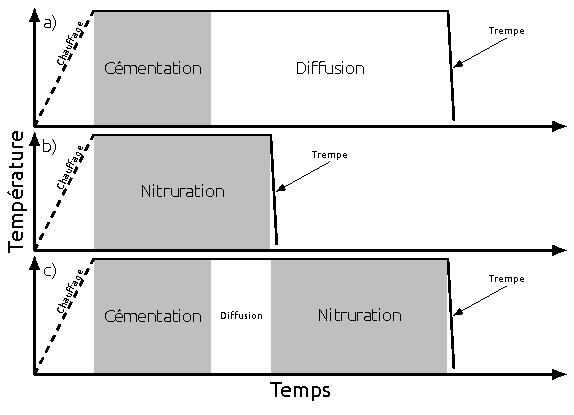
\includegraphics{figures/ch-04-heat_cycles}}
  
  \caption{\label{fig:heat-cycles}Représentation graphique des cycles thermiques des traitements d'enrichissement à \SI{1173}{\kelvin} définis dans le Tableau~\ref{tab:treatment-conditions}: a) cémentation, b) nitruration et c) carbonitruration. Les traitements de revenu ne sont pas représentés.}
\end{figure}

Finalement, pour atteindre les propriétés mécaniques envisagées, tous les traitements ont été suivis d'une trempe à l'huile à la température ambiante \textendash{} soit environ \SI{298}{\kelvin} \textendash{} et d'un traitement cryogénique dans l'azote liquide en ébullition \textendash{} à \SI{77}{\kelvin}. Après le traitement cryogénique, les échantillons ont été soumis à un revenu soit de \SI{18}{\hour} à \SI{573}{\kelvin}, soit de \SI{70}{\hour} heures à \SI{453}{\kelvin}. Le revenu à plus haute température doit permettre l'étude de la stabilité des couches dans des conditions sévères d'opération, alors que le revenu correspond à l'approche classiquement employée avec ce type de traitements thermochimiques. Dans le cas de la nitruration austénitique, un revenu pendant \SI{18}{\hour} à \SI{673}{\kelvin} a aussi été réalisé.

\subsection{Caractérisation des échantillons}
\label{sec:caracterisation_materiaux}

Les échantillons traités dans les conditions décrites à la section précédente pour l'étude des propriétés mécaniques et métallurgiques ont été caractérisés par microscopie optique (MO), microscopie électronique en transmission (MET) et micro-dureté Vickers (HV). Pour les analyses MO et HV, les échantillons ont été enrobés dans une résine époxy et préparés par polissage au papier abrasif jusqu'à une taille de particule inférieure à \SI{14}{\micro\metre}, étape qui a été suivie par un polissage au moyen d'une suspension en alumine jusqu'à une taille de particules inférieure à \SI{0,01}{\micro\metre}. Les indentations Vickers ont été réalisées avec une charge de \SI{300}{gf}. Les profils de diffusion ont été déterminés en employant une micro-sonde électronique Jeol-JXA-8530F. Une procédure similaire à celle qui vient d'être décrite a été adoptée pour la préparation des échantillons servant à la détermination des profils de diffusion mais dans ce cas la résine d'enrobage a été remplacée par un alliage métallique à bas point de fusion ($\approx\SI{353}{\kelvin}$) pour assurer une meilleure conductivité requise par les analyses. Les mesures ont été réalisées tous les \SI{25}{\micro\metre} et la quantification des résultats s'est faite selon la méthode d'étalonnage décrite par \citet{Catteau2014} (en utilisant du $\gamma^{\prime}$\ch{Fe4N} st{\oe}chiométrique pour l'azote et la méthode de la courbe de calibration proposée par \cite{Robaut2006} pour le carbone).

Dans le cas de la microscopie en transmission, réalisée sous un potentiel de \SI{200}{\kilo\volt}, les lames minces ont été prélevées à une distance fixe de \SI{100}{\micro\metre} de la surface traitée. Les lames ont été préparées par la technique FIB~\footnote{de l'anglais \textit{Focused Ion Beam}, Sonde Ionique Focalisée, voir \citet{Williams2009}.} et par polissage manuel des lames jusqu'à une épaisseur inférieure à \SI{50}{\micro\metre} suivi d'une attaque électrolytique. Le MET a été employé pour l'identification des précipités par microanalyse chimique qui permet l'établissement de cartographies de composition par EDX~\footnote{de l'anglais \textit{Energy Dispersive X-ray}, Analyse Dispersive en Énergie, voir \citet{Williams2009}.}. La spectrométrie de pertes d'énergie des électrons (EELS) a été employée comme moyen plus précis de localisation des éléments interstitiels. Les phases présentes ont été identifiées par diffraction des électrons.

\section{Profils de diffusion et prise de masse}
\label{sec:comparaison_procedes}

Les enrichissements réalisés ont été évalués par mesure de prises de masse et par détermination des profils de diffusion dans les échantillons. À partir de l'intégration des profils mesurés par micro-sonde, la prise de masse par unité de surface peut être estimée selon l'Équation~\ref{eq:mass_gain} (Annexe~\ref{an:integration_diffusion}). Les valeurs ainsi obtenues sont comparées à des simulations réalisées à l'aide de Thermo-Calc~\cite{Andersson2002,Borgenstam2000} et de l'intégration numérique du système simplifié \ch{Fe-C-N} décrit à la Section~\ref{sec:integration_slycke}. Bien que Thermo-Calc~\cite{Andersson2002,Borgenstam2000} prenne en compte la précipitation des nitrures et l'interaction entre les éléments interstitiels et la matrice, l'intérêt de l'approche simplifiée réside dans la possibilité d'une utilisation rapide dans un contexte industriel. L'effet d'interaction entre éléments interstitiels est bien connu~\cite{Bhadeshia1980,Bhadeshia2004,Oda1994,Sozinov1997225,Sozinov1999927} et il doit être pris en compte pour une prédiction fiable des profils de diffusion. On peut montrer, par exemple, que pour simuler une prise de masse intégrant l'équation de la diffusion avec un schéma de Crank-Nicolson~\cite{CrankNicolson1947} à concentration constante et égale à la saturation en surface, le coefficient de diffusion du carbone indépendant de la composition~\cite{Slycke1981ii} doit être multiplié par un facteur de 1,8--2,0 pour obtenir un résultat en accord avec les mesures~\cite{Bhadeshia2004}.

Cette analyse a pour but de vérifier la cohérence entre la méthode macroscopique \textendash{} mesure de variation de masse \textendash{} et microscopique \textendash{} micro-sonde \textendash{} et leur convergence selon les conditions aux limites employées dans les simulations. Plusieurs sources d'écart sont possibles entre ces approches: \begin{inparaenum}[(i)] \item le gain de masse par oxydation de surface, \item l'imprécision de la balance et la mesure de surface des pièces, \item l'état de préparation des surfaces, \item les effets de bord qui affectent l'homogénéité de l'enrichissement, \item l'effet de numéro atomique sur l'absorption des rayons x dans les mesures de sonde, \item l'imprécision des données thermodynamiques, etc. \end{inparaenum} Le Tableau~\ref{tab:mass_gain} présente une comparaison entre ces différentes sources de données pour les études réalisées. Les profils de diffusion mesurés sont présentés Figure~\ref{fig:diffusion_profiles}. Cependant, l'ordre de grandeur des valeurs \og{}mesurées\fg{} et simulées reste proche et l'analyse s'avère utile pour valider les conditions aux limites employées dans les simulations des profils de diffusion.

\begin{table}[h]
  \caption{\label{tab:mass_gain}Comparaison entre les prises de masse mesurées et simulées.}
  
  \footnotesize{}\centering{}
  \begin{tabular*}{\textwidth}{@{\extracolsep{\fill}}lcccc} 
    \toprule[2pt]
    % line 1
    \multirow{2}{*}[-3pt]{\centering\bfseries Traitement} &
    \multicolumn{4}{c}{\bfseries Prise de masse (\si{\gram\per\square\metre})}\\
    %line 2
    \cmidrule(l){2-5} & 
    \multicolumn{1}{p{2.5cm}}{
      \centering\bfseries Mesurée  \\ {\tiny{}(Balance)}} & 
    \multicolumn{1}{p{2.5cm}}{
      \centering\bfseries Intégrée \\ {\tiny{}(Micro-sonde)}} &
    \multicolumn{1}{p{2.5cm}}{
      \centering\bfseries Simulée  \\ {\tiny{}(Thermo-Calc)}} &
    \multicolumn{1}{p{2.5cm}}{
      \centering\bfseries Simulée  \\ {\tiny{}(Annexe~\ref{an:integration_diffusion})}} \\
    \midrule[2pt]
    \multicolumn{5}{c}{Alliage 16NiCrMo13}\\
    \midrule[1pt]
    %line 3
    Cémentation
    & 28,8 & 23,5 & 21,0 & 22,2 \\[6pt]
    %line 5
    Nitruration
    & 6,3 & 5,0 & 6,0 & - \\[6pt]
    %line 6	
    Carbonitruration
    & 22,1 & 21,0 & 22,2 & - \\
    \midrule[2pt]
    \multicolumn{5}{c}{Alliage 23MnCrMo5}\\  
    \midrule[1pt]
    %line 3
    Cémentation
    & 20,5 & 15,3 & 17,6 & 17,6 \\[6pt]
    %line 5
    Nitruration
    & 8,5 & 5,8 & 6,1 & - \\[6pt]
    %line 6	
    Carbonitruration
    & 29,0 & 25,1 & 29,1 & - \\
    \bottomrule 
  \end{tabular*}
\end{table}

\begin{table}[!hb]
	\caption{\label{tab:conditions-sim-diffusion}Conditions aux limites pour la simulation des profils de diffusion réalisées à l'aide de Thermo-Calc~\cite{Andersson2002,Borgenstam2000} et selon Annexe~\ref{an:integration_diffusion} pour les étapes de cémentation et nitruration des traitements thermochimiques. Les étapes de diffusion à flux nul ont été simulées en considérant le système fermé. Un flux $J_{i}$ (où $i=\ch{C},\ch{N}$) positif désigne l'entrée de l'élément dans le matériau. Les activités sont notées $a_{i}^{m}$ et les fractions massiques $w_{i}$.}
	
	\centering{}\footnotesize{}
	\begin{tabular}{lclc}
		\toprule[2pt]
		\multicolumn{1}{c}{\bfseries{}Étape}
		& \textbf{Alliage} 
		& \multicolumn{1}{c}{\bfseries{}Thermo-Calc~\cite{Andersson2002,Borgenstam2000}} 
		& \textbf{Annexe}~\ref{an:integration_diffusion}
		\tabularnewline
		\midrule[2pt]
		\multirow{2}{2cm}[-3pt]{Cémentation}
		& 16NiCrMo13 & $a_{\ch{C}}^{m}=0,85$ & $w_{\ch{C}}=0,0100$
		\tabularnewline[6pt]
		& 23MnCrMo5  & $a_{\ch{C}}^{m}=0,66$ & $w_{\ch{C}}=0,0095$
		\tabularnewline[6pt]
		%
		\multirow{4}{2cm}[-12pt]{Nitruration}
		& \multirow{2}{2cm}[-3pt]{16NiCrMo13} 
		& $J_{\ch{N}}=5\times{}10^{-2}(10-a_{\ch{N}}^{m})~\si{\micro\mole\per\square\metre\per\second}$ & -
		\tabularnewline[6pt]
		& & $J_{\ch{C}}=-6\times{}10^{-4}a_{\ch{C}}^{m}~\si{\micro\mole\per\square\metre\per\second}$ & -
		\tabularnewline[6pt]
		& \multirow{2}{2cm}[-3pt]{23MnCrMo5}  
		& $J_{\ch{N}}=5\times{}10^{-2}(40-a_{\ch{N}}^{m})~\si{\micro\mole\per\square\metre\per\second}$ & -
		\tabularnewline[6pt]
		& & $J_{\ch{C}}=-1\times{}10^{-3}a_{\ch{C}}^{m}~\si{\micro\mole\per\square\metre\per\second}$ & -
		\tabularnewline
		\bottomrule
	\end{tabular}
\end{table}

Les simulations à l'aide de Thermo-Calc~\cite{Andersson2002,Borgenstam2000} ont été réalisées en considérant une activité constante du carbone en surface. Pour reproduire les résultats expérimentaux, une activité légèrement supérieure à celle de saturation à la température de traitement a été employée pour la nuance 16NiCrMo13 et légèrement inférieure pour la nuance 23MnCrMo5, ces écarts étant probablement liés aux variations de la température de point de rosée pendant les expériences. L'état de référence adopté pour le carbone est le graphite et la formation de cémentite n'a pas été prise en compte. De la même façon, une fraction massique égale à 0,010 a été utilisée pour la simulation simplifiée de l'alliage 16NiCrMo13 et 0,0095 pour la nuance 23MnCrMo5, valeurs correspondant aux activités utilisées pour les simulations à l'aide de Thermo-Calc~\cite{Andersson2002,Borgenstam2000}. Ces conditions aux limites sont résumées Tableau~\ref{tab:conditions-sim-diffusion}. Ces simulations se trouvent être en bon accord entre elles et reproduisent l'ordre de grandeur des profils intégrés en utilisant les mesures faites par microsonde pour la cémentation. On doit remarquer que les conditions employées dans ces simulations de l'étape de cémentation ne correspondent pas à l'activité $a_{\ch{C}}^{m}\approx{}1$ associée à la température de point de rosée $T_{r}=\SI{263}{\kelvin}$ établie pour l'atmosphère utilisée (Tableau~\ref{tab:conditions-traitement}). Cependant, des profils similaires peuvent être obtenus en utilisant cette condition $a_{\ch{C}}^{m}\approx{}1$ si l'on considère la précipitation de cémentite en surface.

Dans les cas de la nitruration austénitique et de la carbonitruration, les simulations sont limitées à Thermo-Calc~\cite{Andersson2002,Borgenstam2000}. Comme l'approche simplifiée pour le système \ch{Fe-C-N} ne tient pas compte de la précipitation des nitrures pendant l'enrichissement, la condition à la limite nécessaire pour atteindre les fractions en azote en surface conduit à des prises de masse simulées que ne sont pas réalistes. Ces simulations considèrent comme état de référence pour l'azote \ch{N2} à une pression de \SI{1}{\atm}. En choisissant cet état, l'activité correspondant à la prise de masse pour la nuance 23MnCrMo5 est $a_{N}=40$, soit un $K_{N}=\SI{8,3E-3}{\atm^{-0,5}}$ (voir Figure~\ref{fig:diagrammes_kn}), cette valeur étant en très bon accord avec la valeur $K_{N}=\SI{8,6E-3}{\atm^{-0,5}}$ obtenue Section~\ref{sec:pyrolyse_ammonia} à la pression atmosphérique (Tableau~\ref{tab:conditions-traitement}). Pour l'alliage 16NiCrMo13, une valeur d'activité $a_{N}=10$ a dû être fixée pour reproduire les résultats expérimentaux. On vérifie donc que l'approche thermodynamique adoptée s'applique très bien à l'enrichissement en azote de l'alliage 23MnCrMo5 mais ce n'est pas le cas pour la nuance 16NiCrMo13. Pour des raisons probablement cinétiques, l'atmosphère utilisée a imposé une fraction en azote en surface très inférieure à celle attendue: on trouve Figure~\ref{fig:diffusion_profiles} des fractions massiques en azote inférieures à 0,003 en surface en lieu de 0,009 associée au $K_{N}$ établi par l'atmosphère. 

Pour simuler les profils de diffusion du carbone pendant l'étape de nitruration de la carbonitruration, un coefficient de transfert de matière a été introduit pour incorporer l'effet de la décarburation avec une condition à la limite de flux variable. Pour la nuance 16NiCrMo13, une valeur de $h=\SI{6,0E-4}{\micro\mole\per\square\metre\per\second}$ a été utilisée ($h=\SI{1,0E-03}{\micro\mole\per\square\metre\per\second}$ pour l'alliage 23MnCrMo5). Les expressions pour les flux de nitruration et décarburation sont fournies Tableau~\ref{tab:conditions-sim-diffusion}. Si l'on considère que le taux de décarburation est plus important si la recombinaison de l'hydrogène adsorbé est moins rapide (et donc la probabilité de formation d'un radical \ch{CH} est augmentée), la relation qualitative entre ces valeurs est en accord avec les profils de diffusion de l'azote: l'alliage 16NiCrMo13 a un effet catalytique sur la recombinaison des produits de craquage de l'ammoniac et donc est moins sensible à la nitruration et à la décarburation. La Figure~\ref{fig:diffusion_profiles} compare également des profils de diffusion simulés pour la carbonitruration et pour la cémentation aux résultats expérimentaux.

\clearpage

\begin{figure}[!ht]
	\centering
	\subfloat[Alliage 16NiCrMo13.]{
		\centering\resizebox{0.48\textwidth}{!}{
			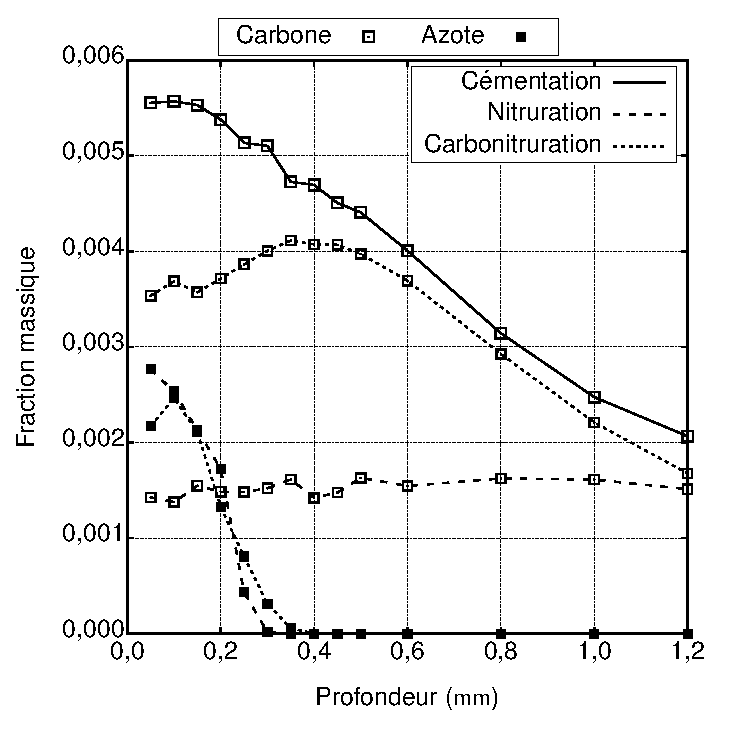
\includegraphics{figures/ch-04-profil_diffusion_aero}}
	}\hfill
	\subfloat[Alliage 23MnCrMo5.]{
		\centering\resizebox{0.48\textwidth}{!}{
			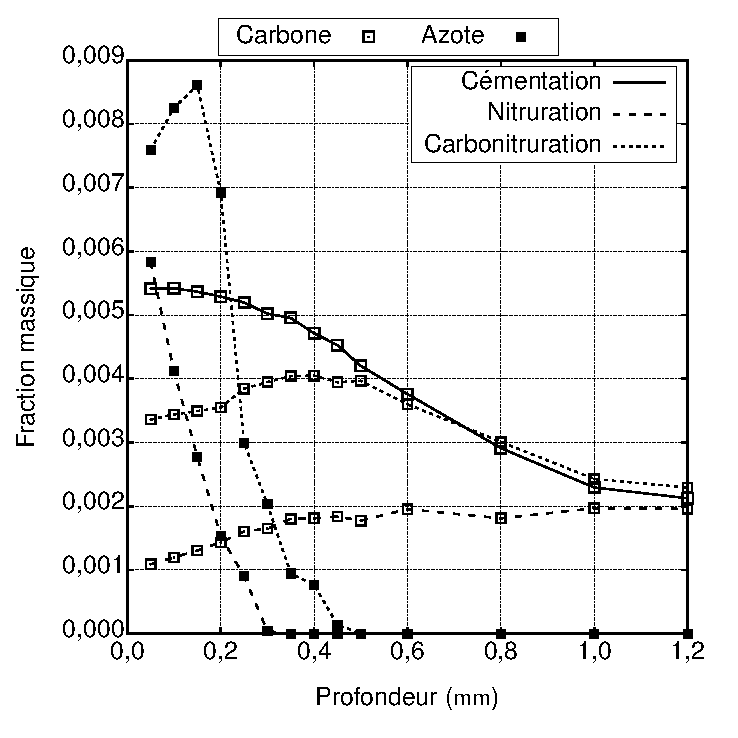
\includegraphics{figures/ch-04-profil_diffusion_auto}}
	}\\
	\subfloat[Simulation alliage 16NiCrMo13.]{
		\centering\resizebox{0.48\textwidth}{!}{
			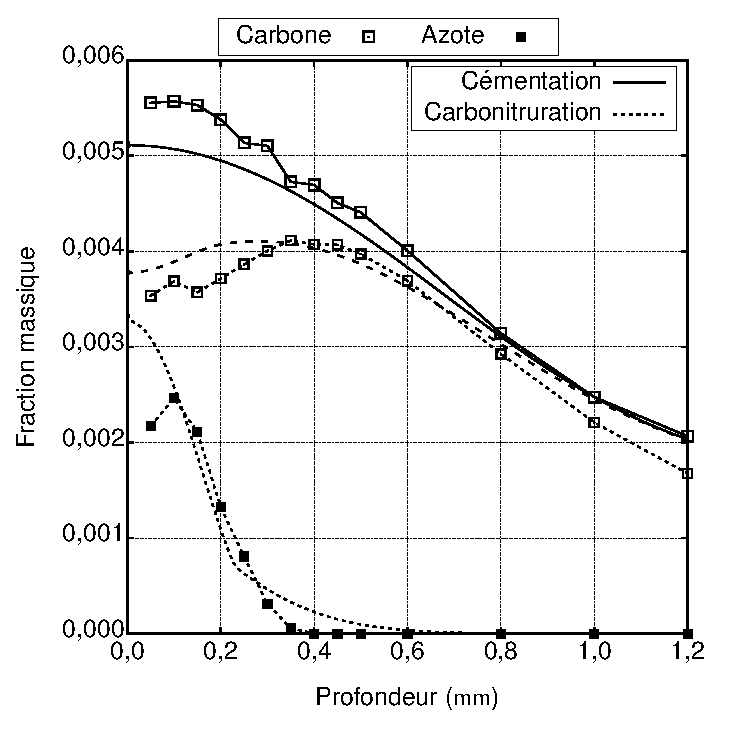
\includegraphics{figures/ch-04-profil_diffusion_sim_aero}}
	}\hfill
	\subfloat[Simulation alliage 23MnCrMo5.]{
		\centering\resizebox{0.48\textwidth}{!}{
			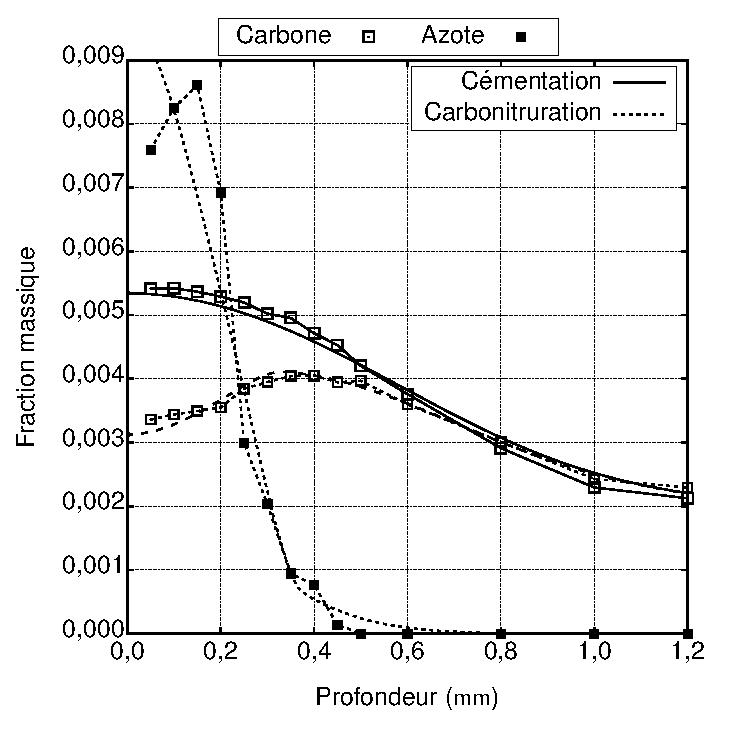
\includegraphics{figures/ch-04-profil_diffusion_sim_auto}}
	}
	
	\caption{\label{fig:diffusion_profiles}Profils de diffusion du carbone et de l'azote après cémentation, nitruration et carbonitruration. Comparaison entre des simulations et mesures expérimentales pour la cémentation et la carbonitruration.}
\end{figure}

\section{Réponses mécaniques}
\label{sec:reponses_mecaniques}

\subsection{Réponse à la trempe}

L'introduction de carbone et d'azote en solution solide permet une diminution de la température de début de transformation martensitique. Par conséquent, la teneur en austénite résiduelle augmente de façon exponentielle \textendash{} comme décrit par l'Équation~\ref{eq:koistinen} attribuée à \citet{Koistinen1959} \textendash{} dans la région traitée. Dans cette étude, on se concentre uniquement sur la réponse mécanique de la martensite, en essayant de minimiser l'austénite résiduelle par une séquence trempe huile -- traitement cryogénique dans l'azote en ébullition. La Figure~\ref{fig:cryogenic_effect_aero} met en évidence le rôle de cette trempe en deux étapes sur la transformation $\gamma_{R}\rightarrow\alpha^{\prime}$ de l'austénite résiduelle $\gamma_{R}$ en martensite $\alpha^{\prime}$ dans une région contenant une fraction massique comprise entre 0,007 et 0,009 en carbone et jusqu'à 0,001 en azote. Figure~\ref{fig:residual-austenite}, on quantifie par analyse d'images une fraction d'environ 35\% d'austénite résiduelle~\footnote{Analyse d'images par conversion de l'image en noir et blanc à travers d'une seuillage des gris manuelle et calcul du rapport des surfaces (en pixels) des zones blanches et de l'image entière.}. Les discussions qui suivent concernent donc des microstructures comme celle de la Figure~\ref{fig:martensite-no-residual}. Dans nos traitements, en général la teneur totale en interstitiels dans les pièces traitées reste en dessous d'une fraction massique d'environ 0,0055, le point-H~\cite{Sherby2008}, et donc les microstructures de départ après trempe huile (\SI{298}{\kelvin}) sont déjà limitées en austénite résiduelle. Ce n'est qu'à partir de cette composition associée au point-H~\cite{Sherby2008} que la fraction en $\gamma_{R}$ devient importante.

\begin{figure}[!h]
  \centering
  \subfloat[\label{fig:residual-austenite}Après trempe huile.]{
    \centering\resizebox{0.48\textwidth}{!}{
    \begin{tikzpicture}
    \node[anchor=south west,inner sep=0] (image1) at (0.0,0.0) {
      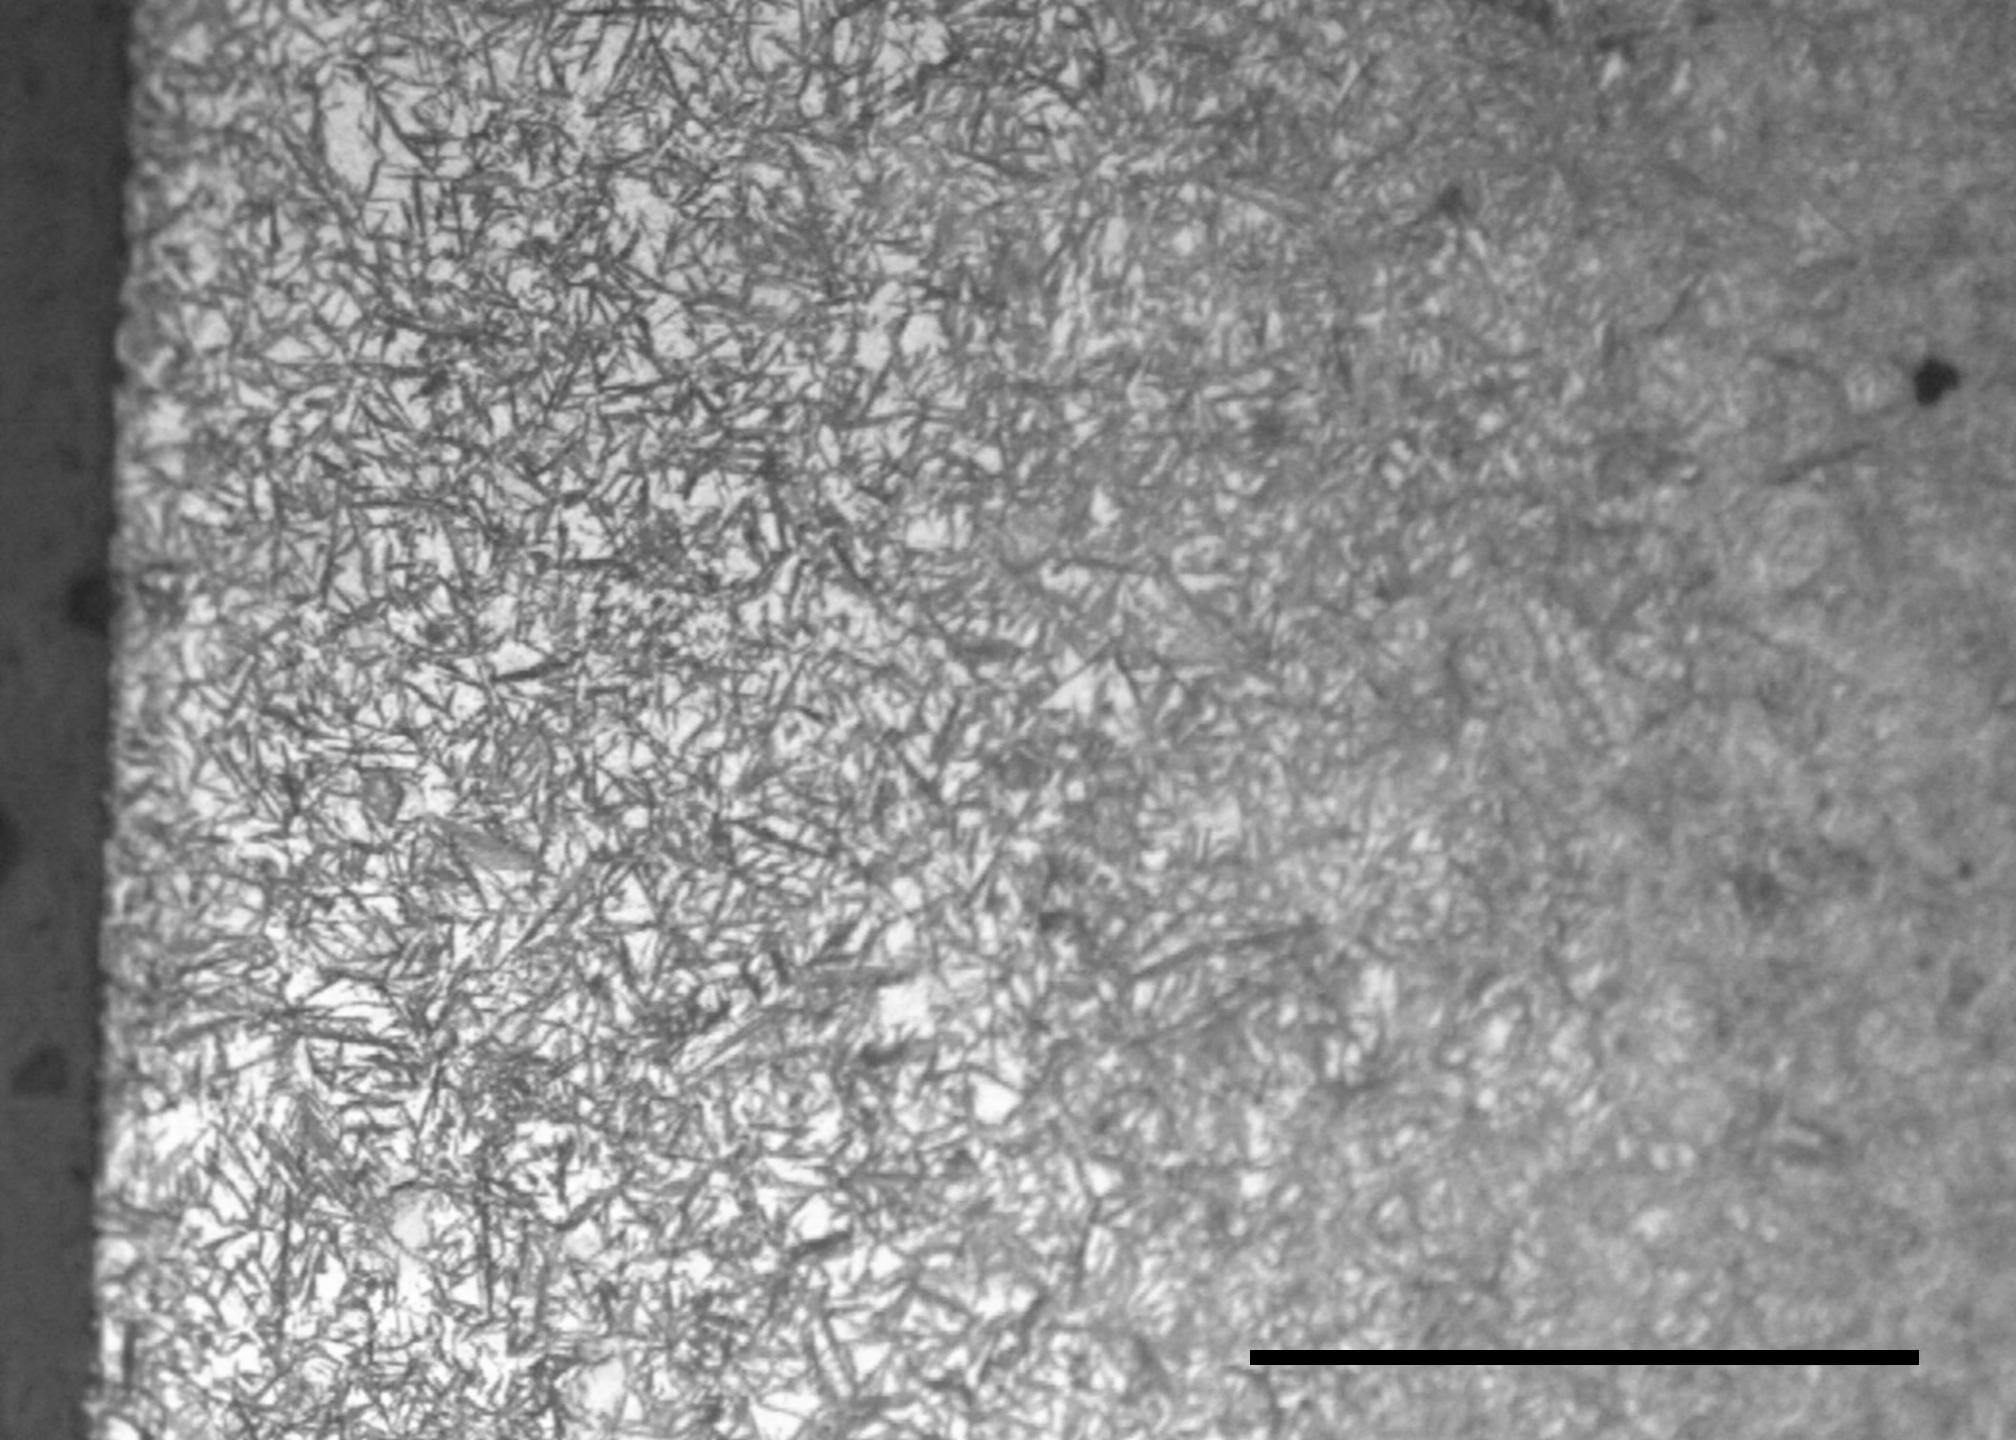
\includegraphics[scale=0.1]{figures/ch-04-aero_carbonitriding_200x_oil}};
    \begin{scope}[x={(image1.south east)},y={(image1.north west)}] 
      \node at (0.8,0.1) {\small\SI{200}{\micro\metre}};
      \node at (0.74, 0.61) {%
        \setlength{\fboxsep}{0pt}
        \setlength{\fboxrule}{2pt}
        \fbox{%
        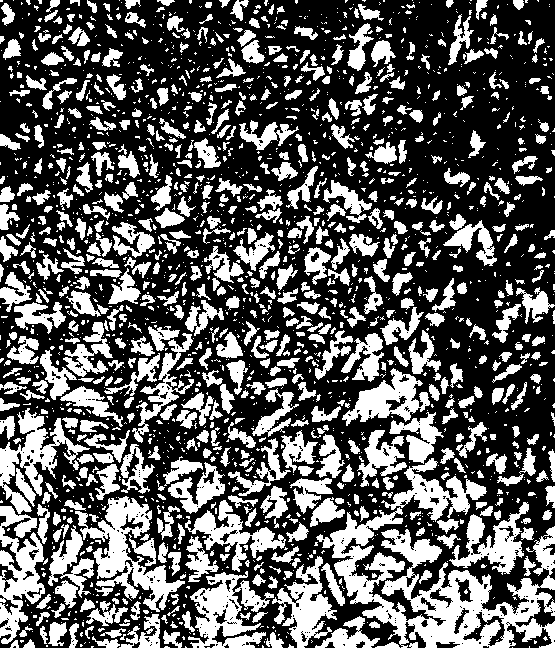
\includegraphics[width=0.2\textwidth]
          {figures/ch-04-aero_carbonitriding_200x_oil_analysis}}
      };
    \end{scope}
    \end{tikzpicture}}
  }\hfill
  \subfloat[\label{fig:martensite-no-residual}Après traitement cryogénique.]{
    \centering\resizebox{0.48\textwidth}{!}{
    \begin{tikzpicture}
    \node[anchor=south west,inner sep=0] (image1) at (0.0,0.0) {
      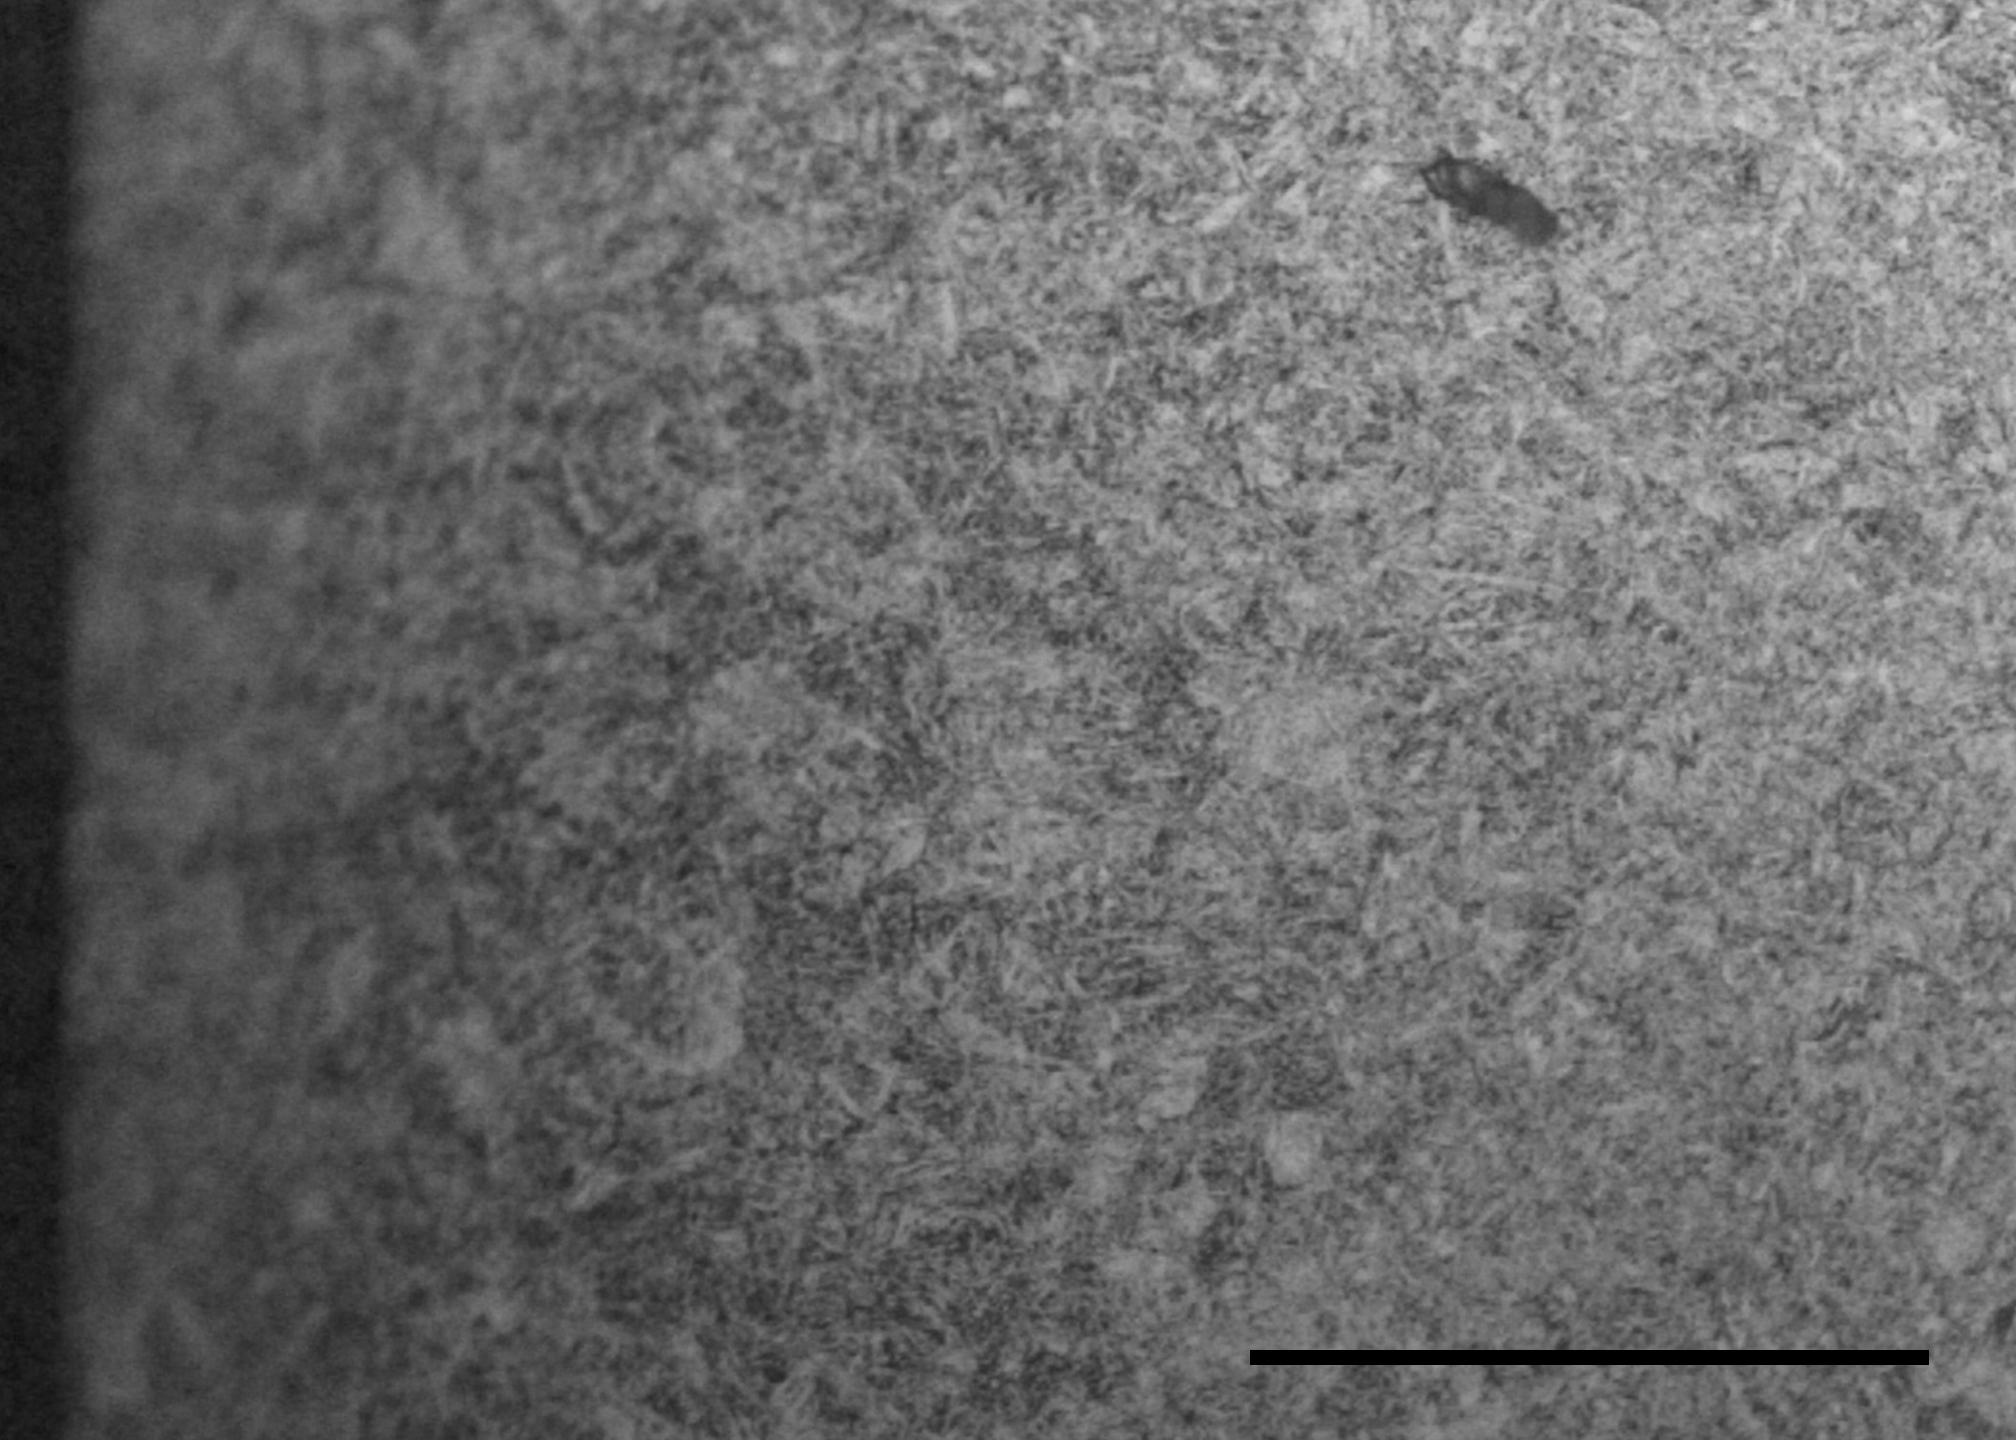
\includegraphics[scale=0.1]{figures/ch-04-aero_carbonitriding_200x_cryo}};
    \begin{scope}[x={(image1.south east)},y={(image1.north west)}] 
    \node at (0.8,0.1) {\small\SI{200}{\micro\metre}};
    \end{scope}
    \end{tikzpicture}}
  }
  
  \caption{\label{fig:cryogenic_effect_aero}Microstructure de l'alliage 16NiCrMo13 enrichi par une fraction massique en carbone donnée en surface après trempe à l'huile à température ambiante et après traitement cryogénique. Microscope optique en lumière visible \textendash{} grandissement de 200$\times$. Le détail à droite de la Figure~\ref{fig:residual-austenite} présente l'image utilisée pour la quantification de $\gamma_{R}$.}
\end{figure}

Les filiations de dureté de la martensite à l'état trempé sont présentées Figure~\ref{fig:hardness_as_quenched} et se trouvent être en bon accord avec des valeurs typiques rapportées dans la littérature~\cite{Grange1977,Krauss1999,Hutchinson20115845,Ferro2014} pour la martensite \ch{Fe-C} et des aciers faiblement alliés. On vérifie Figure~\ref{fig:hardness_as_quenched} le comportement complémentaire du carbone et de l'azote dans l'établissement de la dureté après trempe: la dureté est conservée comme celle de la cémentation en surface des pièces carbonitrurées malgré la décarburation mise en évidence pendant l'introduction de l'azote, ce qui montre la capacité de cet élément à substituer le carbone. En extrême surface (\SI{0,2}{\milli\metre}) de l'alliage 16NiCrMo13, on met en évidence une chute de dureté pour les deux traitements qui est plus prononcée pour la carbonitruration. Cela peut s'expliquer par la formation d'austénite résiduelle~\footnote{À partir de l'Équation~\ref{eq:koistinen}, on montre que pour une teneur en carbone et une température de trempe données, le rapport $r_{\gamma_{R}}$ entre les fractions volumiques d'austénite résiduelle prédites pour les alliages 16NiCrMo13 et 23MnCrMo5 est donnée par $r_{\gamma_{R}}=\exp\big[-1,1\times 10^{-2}(M_{s,\mathrm{16NiCrMo13}}-M_{s,\mathrm{23MnCrMo5}})\big]$. Si l'on considère, par exemple, la formule d'\citet{Andrews1965} pour le calcul de la température d'initiation de la réaction martensitique $M_s$ pour chaque alliage en fixant une teneur en carbone, on montre que ce rapport est de l'ordre de 1,4 -- l'alliage 16NiCrMo13 retient 40\% d'austénite résiduelle de plus que la nuance 23MnCrMo5.}. 
On a présenté Section~\ref{sec:martensite_cn} le modèle de durcissement utilisé pour expliquer la réponse à la trempe dans notre cas: la dureté de la martensite doit augmenter de façon linéaire avec la racine carrée de la fraction molaire $x_{i}$ en interstitiels dissous. On applique le raisonnement de \citet{Hutchinson20115845} qui suppose que les atomes interstitiels en solution solide se comportent comme des agglomérats capables de bloquer le mouvement des dislocations, ces agglomérats contribuent à augmenter la résistance mécanique selon une dépendance en racine carrée de leur teneur~\cite{Haasen19962009}. Comme évoqué par les auteurs~\cite{Hutchinson20115845}, ces atomes ne sont pas nécessairement dans les sites octaédriques de la martensite, mais dans les défauts cristallins sous forme d'atmosphères de Cottrell, stoppant le glissement des dislocations. Par ailleurs, \citet{Morito20031475} montrent une dépendance linéaire entre la teneur en carbone et la densité de dislocations $\rho$ qui augmente aussi en racine carrée la résistance mécanique des alliages~\cite{Cohen1968,Norstrom1976,Krauss1999,Hutchinson20115845}. On a donc ces deux phénomènes complémentaires produisant la réponse en dureté de la martensite trempée selon un même type de dépendance: la racine carrée de la teneur en interstitiels dissous. 

\begin{figure}[h]
  \subfloat[Alliage 16NiCrMo13.]{
    \centering\resizebox{0.48\textwidth}{!}{
      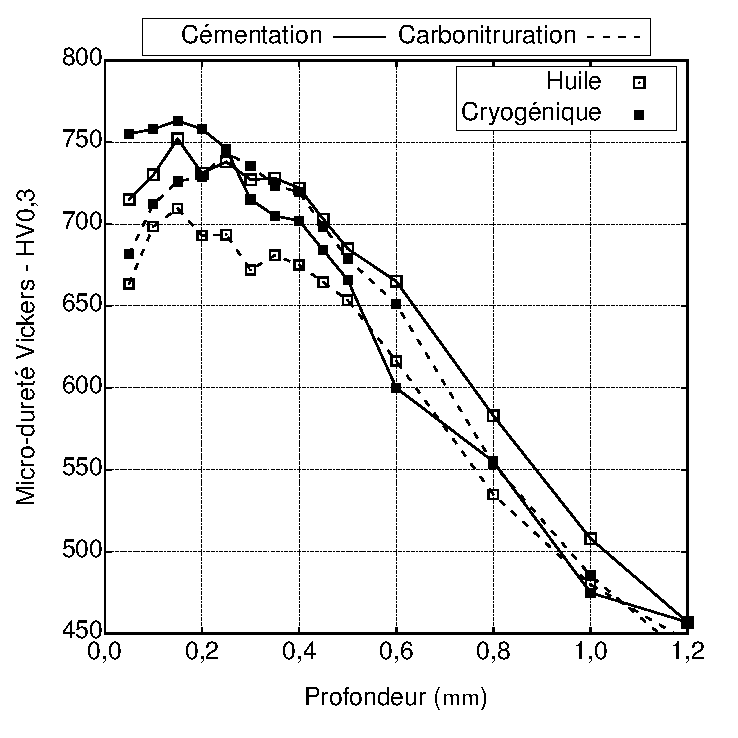
\includegraphics{figures/ch-04-hardness_as_quenched_aero}}
  }\hfill
  \subfloat[Alliage 23MnCrMo5.]{
    \centering\resizebox{0.48\textwidth}{!}{
      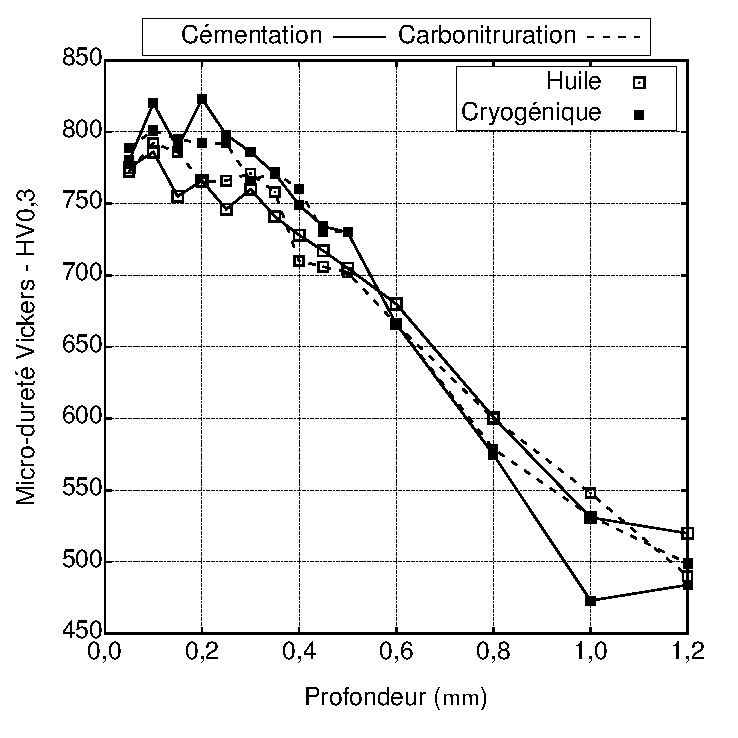
\includegraphics{figures/ch-04-hardness_as_quenched_auto}}
  }

  \caption{\label{fig:hardness_as_quenched}Dureté après cémentation et carbonitruration suivies d'une trempe à l'huile et traitement cryogénique en fonction de la distance à la surface des pièces traitées.}
\end{figure}

On fait l'hypothèse que ce comportement peut aussi être attribué à l'azote en solution solide en dessous du point-H~\cite{Sherby2008}, i.e. dans la région du domaine martensitique cubique, à partir duquel la croissance rapide de la teneur en austénite résiduelle s'écarte de la réponse linéaire de la limite élastique avec la racine carrée en interstitiels. On généralise la relation proposée par \citet{Cohen1968,Norstrom1976} en ajoutant la dépendance avec la fraction en azote. Il est clair que cette approche n'est possible que si l'on utilise des fractions molaires $x_{i}$, avec $i = (\ch{C},\ch{N})$: c'est le nombre d'atomes en solution qui constitue la variable régissant la limite élastique. Cette hypothèse faite, il nous est nécessaire de connaître l'azote dissous en solution solide. C'est là que réside l'importance de l'utilisation de Thermo-Calc~\cite{Andersson2002,Borgenstam2000} et de l'obtention de profils de diffusion simulés en bon accord avec les mesures expérimentales: une allure \og{}correcte\fg{} du profil de diffusion de l'azote simulée traduit une prédiction \og{}correcte\fg{} des nitrures formés pendant l'enrichissement en azote et donc une bonne valeur de l'azote en solution solide qui pourra être utilisée dans le modèle de durcissement. 

Il faut remarquer que la précision des profils de diffusion n'a pas de lien direct avec l'adéquation des conditions aux limites. Comme on l'a montré Section~\ref{sec:comparaison_procedes}, l'activité de l'atmosphère ne correspond pas à la teneur en surface obtenue dans l'alliage 16NiCrMo13, bien que le profil de diffusion simulé pour $a_{N}=10$ semble décrire correctement l'allure des mesures réalisées par EPMA sur la Figure~\ref{fig:diffusion_profiles}: on suppose donc que la prédiction du comportement de l'azote en diffusion-précipitation est correcte, la condition aux limites étant différente de celle fournie par la thermodynamique de l'atmosphère. En fonction de ces résultats, Thermo-Calc~\cite{Andersson2002,Borgenstam2000} a été utilisé pour simuler la teneur en interstitiels en solution solide pour chaque point rapporté Figure~\ref{fig:diffusion_profiles}. D'autres contributions, i.e. durcissement par solution solide promu par les éléments d'alliage, morphologie de la martensite, etc. sont ici considérés comme négligeables. La Figure~\ref{fig:hardness_norstrom} présente la dépendance de la dureté (ici supposée proportionnelle à la limite élastique) avec $x_{i}^{0.5}$, la racine carrée de la fraction molaire totale d'éléments interstitiels en solution solide. 

Les éléments carbone et azote sont considérés comme possédant une capacité de blocage des dislocations similaires du fait de leur taille dans l'austénite: l'azote possède un rayon environ 5-7\% supérieur à celui du carbone~\cite{Yahia1995}. Une étude exhaustive pourrait permettre l'introduction d'un coefficient pour chaque élément, ce qui n'a pas été fait ici. On observe deux régions principales Figure~\ref{fig:hardness_norstrom}, la première à gauche de $\mathrm{x_{i}^{0,5}=0,16}$, où le modèle de \citet{Norstrom1976} est valable et la dureté augmente de façon linéaire avec le paramètre $x_{i}^{0,5}$ puis, la seconde au-delà de cette limite où l'on trouve un plateau de durcissement et même une chute en dureté pour des fractions plus élevées en interstitiels. Un deuxième axe est ajouté en haut de la Figure~\ref{fig:hardness_norstrom} pour donner la fraction massique estimée correspondant à chaque $x_{i}^{0,5}$, la conversion précise n'étant pas possible en raison des différentes masses des éléments en solution. Le point-H~\cite{Sherby2008} est identifié sur la figure, indiquant la limite pratique d'amélioration de la limite élastique des surfaces des aciers faiblement alliés sans que des traitements cryogéniques soient réalisés. À partir de $x_{i}^{0,5}=0,18$ une chute importante en dureté est mise en évidence pour l'alliage 16NiCrMo13 en raison de la présence de l'austénite résiduelle. Sa décomposition rend possible l'augmentation de la dureté au niveau du plateau formé à \SI{850}{\HV}. 

\begin{figure}[h]
  \centering
  \resizebox{0.98\textwidth}{!}{
    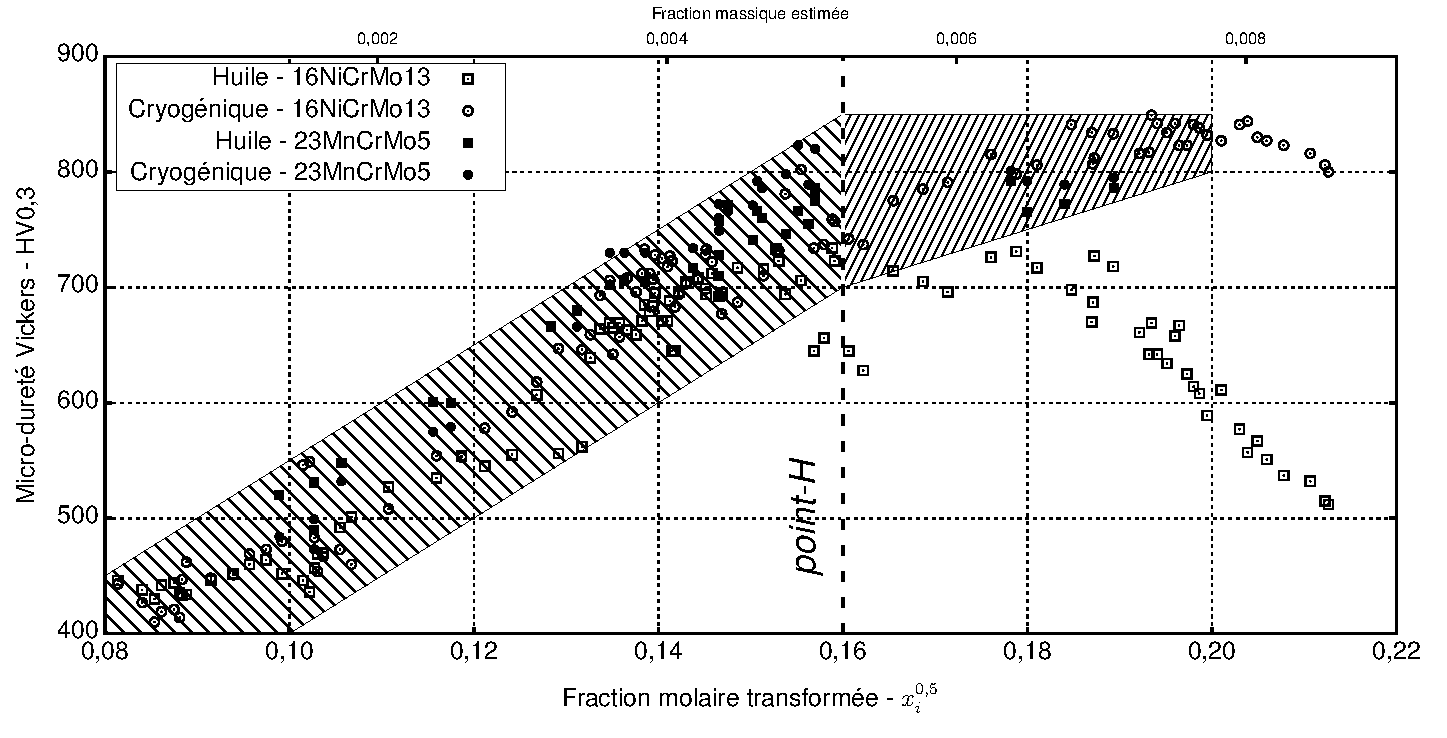
\includegraphics{figures/ch-04-hardness_norstrom}}
  
  \caption{\label{fig:hardness_norstrom}Dureté après trempe à l'huile et traitement cryogénique en fonction de la racine carrée de la somme des fractions molaires en carbone et en azote en solution solide juste avant trempe.  Les données d'entrée pour l'azote sont issues de simulations à l'aide de Thermo-Calc~\cite{Andersson2002,Borgenstam2000}. Les points sont issus de toutes les gammes de traitement réalisées, sans faire la distinction entre les enrichissements par un élément interstitiel spécifique.}
\end{figure}

\subsection{Réponse au revenu}

Bien que la dureté à l'état trempé puisse être expliquée par la composition locale, le revenu induit une série de processus plus complexes conduisant normalement à une chute de dureté sur toute la profondeur enrichie, comme cela est présenté Figure~\ref{fig:hardness_temper} pour la cémentation et la carbonitruration \textemdash{} l'état de référence choisi correspond à la dureté obtenue après traitement cryogénique. Une chute en dureté moins importante est observée pour la carbonitruration sur la zone enrichie en azote \textendash{} voir Figure~\ref{fig:diffusion_profiles} \textendash{} si on la compare à la cémentation, effet qui est particulièrement prononcé pour les deux conditions de revenu de l'alliage 23MnCrMo5. Dans ce cas, même si la dureté de départ \textendash{} après traitement cryogénique \textendash{} est de l'ordre de \SI{800}{\HV} pour les deux traitements thermochimiques, les profils enrichis en azote préservent un gain en dureté sur une profondeur de \SI{0,3}{\milli\metre} d'environ \SI{70}{\HV} par rapport à la dureté à c{\oe}ur.

\begin{figure}[h]
  \centering
  \subfloat[Alliage 16NiCrMo13.]{
    \centering\resizebox{0.48\textwidth}{!}{
    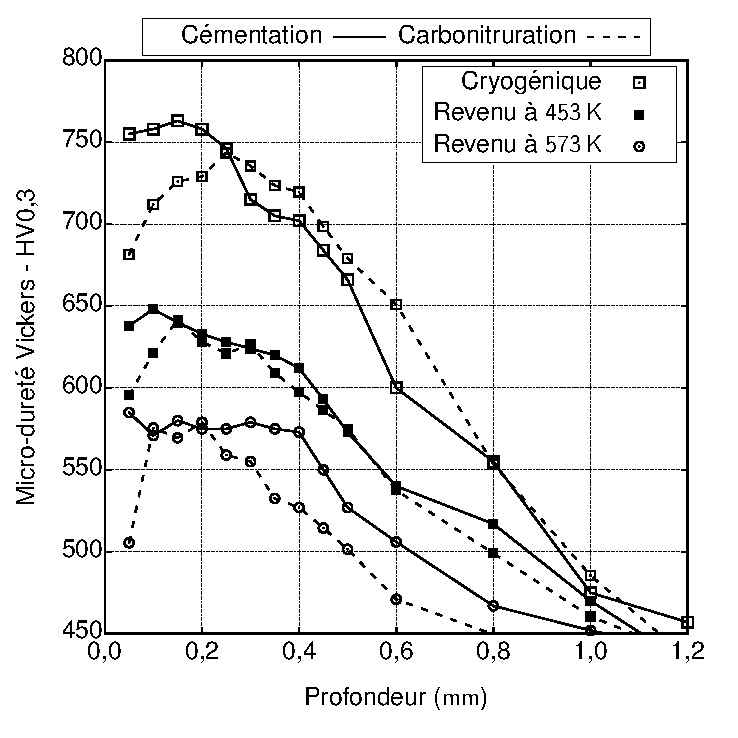
\includegraphics{figures/ch-04-hardness_temper_aero}}
  }\hfill
  \subfloat[Alliage 23MnCrMo5.]{
    \centering\resizebox{0.48\textwidth}{!}{
    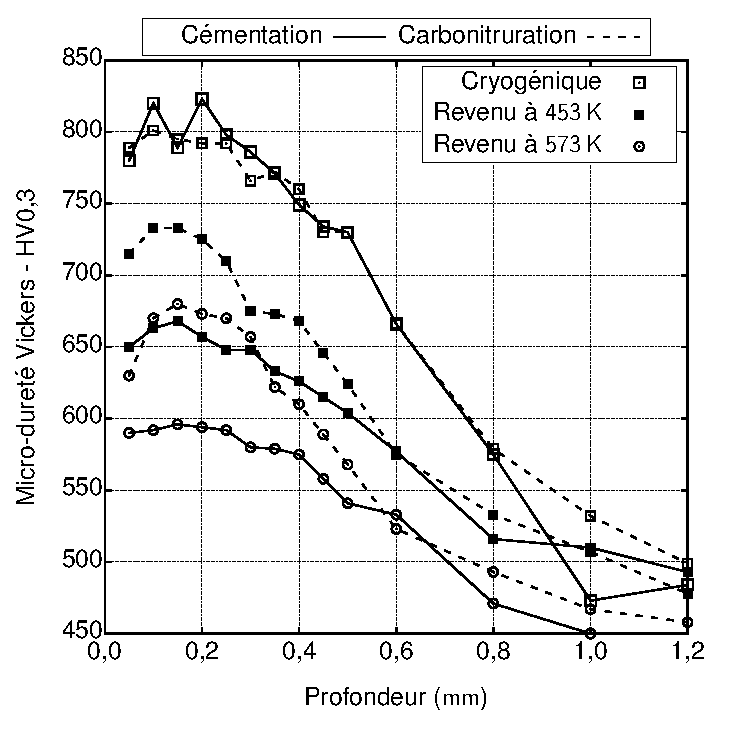
\includegraphics{figures/ch-04-hardness_temper_auto}}
  }
  
  \caption{\label{fig:hardness_temper}Dureté après cémentation et carbonitruration suivies soit d'un traitement cryogénique soit d'un revenu en fonction de la distance à la surface des pièces traitées.}
\end{figure}

L'alliage 23MnCrMo5 a été enrichi à environ 0,8~\%~N en poids en surface. Si l'on considère la formation de nitrures de type \ch{MN}, cela devrait réduire le chrome en solution à moins de 0,3~\% en poids et une martensite moins stable au revenu est alors attendue~\cite{Grange1977}. Comme cela a été montré par \citet{Catteau2016}, même pour des teneurs plus faibles en azote, cet alliage devrait précipiter aussi des nitrures mixtes \ch{MnSiN2}, qui devrait accroître d'autant l'appauvrissement de la matrice en éléments carburigènes capables de retarder la cinétique de revenu par la précipitation de carbures. On observe Figure~\ref{fig:microstructure-auto-quenched} une forte densité de particules submicrométriques \textendash{} elles seront caractérisées par microscopie électronique en transmission \textendash{} sur une profondeur de \SI{300}{\micro\metre}. Par conséquent, le revenu de cet alliage doit être gouverné par une matrice moins riche en éléments d'alliage et doit présenter un comportement proche de celui du fer pur, pour lequel une précipitation de \ch{Fe16N2} cohérent à basse température est attendue. Ce type de précipité devient incohérent dans les premiers instants du revenu et est finalement converti à l'équilibre en \ch{Fe4N}~\cite{Kaplow1983,vanGent1985,Mittemeijer1988,Cheng199013,Cheng19902857,Fall1996,vanGenderen1997}. Cette séquence ne peut pas expliquer les réponses mécaniques obtenues: on peut alors penser soit à une \og{} dureté composite \fg{} entre la matrice et les précipités présents à forte concentration, soit à une transformation retardée par présence d'éléments d'alliage, la phase \ch{Fe16N2} cohérente pouvant alors apporter un durcissement comme dans le cas du système \ch{Fe-N}~\cite{Mittemeijer2010}. 

\begin{figure}[h]
  \resizebox{0.98\textwidth}{!}{
    \iftoggle{paper}
    {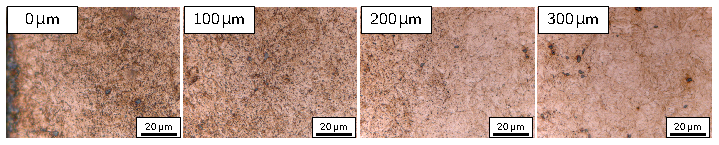
\includegraphics{figures/ch-04-micrograph_auto_quenched-pdf}} % print
    {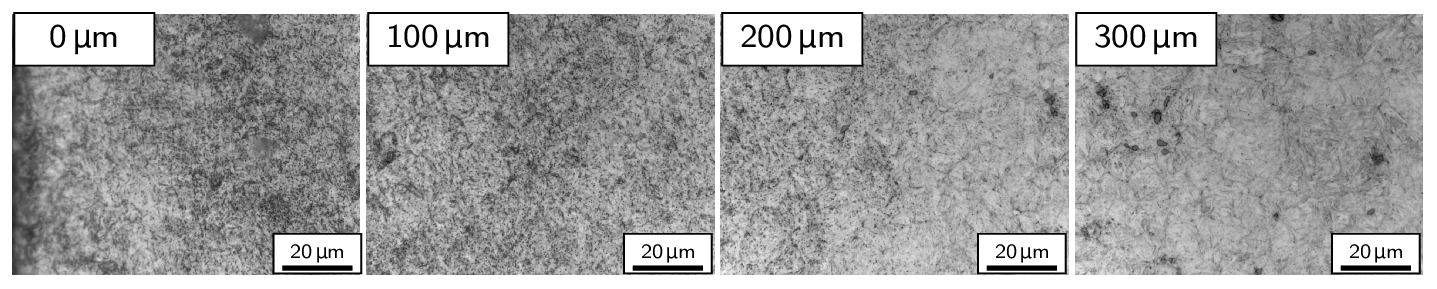
\includegraphics{figures/ch-04-micrograph_auto_quenched-png}} % digital
  }
  
  \caption{\label{fig:microstructure-auto-quenched}Gradient de précipités formés pendant l'enrichissement de l'alliage 23MnCrMo5 carbonitruré. On observe une forte densité de points sombres sur les micrographies à \SI{0}{\micro\metre} et à \SI{100}{\micro\metre} suivi d'une décroissance jusqu'à une microstructure majoritairement martensitique à \SI{100}{\micro\metre}.  Microscope optique en lumière visible \textendash{} grandissement de 1250$\times$.}
\end{figure}

\subsection{Réponse à la nitruration}

Les réponses mécaniques à la nitruration austénitique sont traitées à part dans cette section relativement au comportement mis en évidence: alors que les enrichissements uniquement en carbone ou combinés carbone-azote ont conduit a une chute en dureté sur toute la profondeur enrichie lors du revenu, les échantillons nitrurés montrent un maintien de la dureté proche de celle de l'alliage trempé si la température de revenu est supérieure à \SI{573}{\kelvin}. Le revenu équivalent determiné à partir du paramètre d'Hollomon \textendash{} constante d'Hollomon-Jaffe supposée égale à 20~\cite{Wan2005,Steel2006} \textendash{} est plus important avec le traitement réalisé à \SI{573}{\kelvin} (\SI{18}{\hour}) par rapport à celui fait à \SI{453}{\kelvin} (\SI{70}{\hour}). De cette façon, un revenu plus prononcé des matériaux était attendu à \SI{573}{\kelvin}, ce qui n'est pas le cas sur toute la profondeur enrichie en azote \textemdash{} Figure~\ref{fig:hardness_nitriding}. 

\begin{figure}[!b]
  \centering
  \subfloat[Alliage 16NiCrMo13.]{
    \centering\resizebox{0.48\textwidth}{!}{
      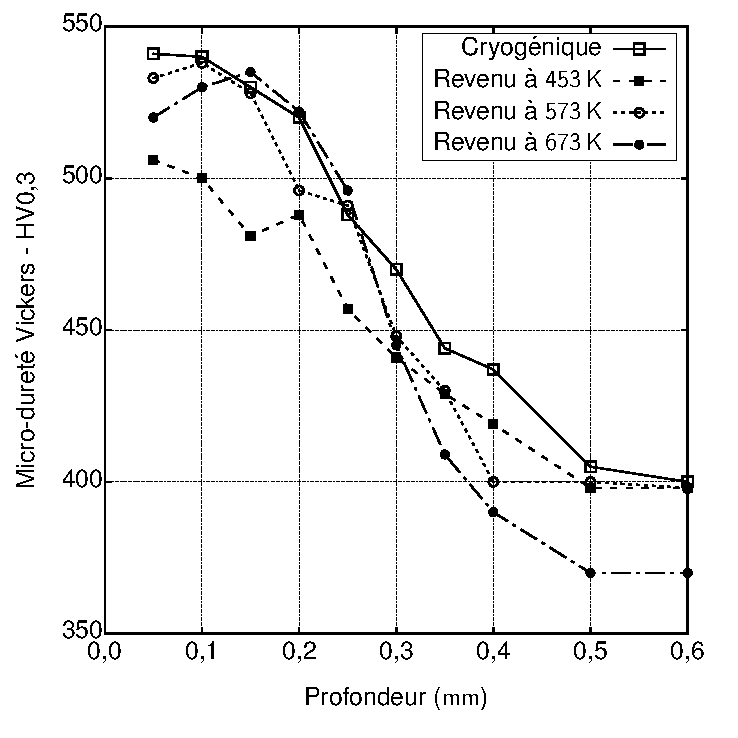
\includegraphics{figures/ch-04-hardness_nitriding_aero}}
  }\hfill
  \subfloat[Alliage 23MnCrMo5.]{
    \centering\resizebox{0.48\textwidth}{!}{
      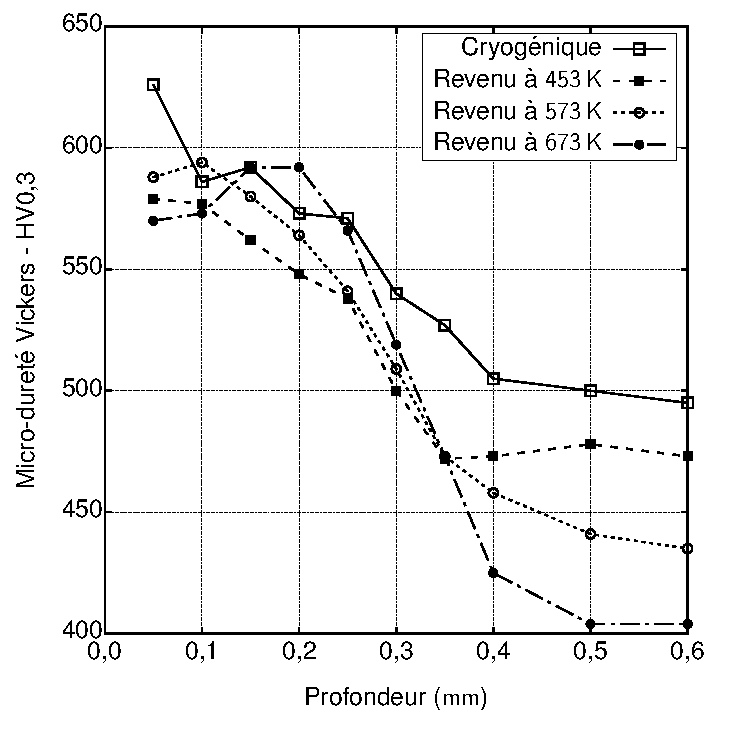
\includegraphics{figures/ch-04-hardness_nitriding_auto}}
  }
  
  \caption{\label{fig:hardness_nitriding}Dureté après nitruration suivie soit par un traitement cryogénique, soit par un traitement cryogénique et un revenu en fonction de la distance à la surface des pièces.}
\end{figure}

La confirmation du phénomène se fait en réalisant un revenu à \SI{673}{\kelvin} pendant \SI{18}{\hour}. La dureté ainsi obtenue est conservée proche de celle après trempe en surface, ce qui peut être lié à une précipitation secondaire. On observe un déplacement du maximum de dureté vers le c{\oe}ur des pièces, ce qui est lié à la coalescence/transition cohérent-incohérent en extrême surface des précipités formés et à la mobilité atomique \textendash{} diffusion de l'azote vers le c{\oe}ur \textendash{}. Finalement, la dureté dans la zone non-nitrurée chute de manière plus importante qu'à plus faible température \textemdash{} en augmentant la température de revenu on diminue progressivement la dureté de la zone au-delà de \SI{0,3}{\milli\metre}. Cette séquence est valable pour les deux alliages étudiés et est plus prononcée pour la nuance 16NiCrMo13, ce qui est possiblement lié à la plus faible teneur en carbone \textendash{} ce comportement n'a pas été mis en évidence lors de la carbonitruration des alliages. Ce comportement peut permettre de comprendre l'amélioration de la résistance au revenu produite par la carbonitruration.

\section{Identification des précipités}
\label{sec:precipitation}

Suite aux résultats de la Section~\ref{sec:reponses_mecaniques}, une étude en  microscopie électronique en transmission ont été réalisées. L'étude vise tout d'abord à identifier les précipités formés à haute température lors des traitements thermochimiques, ce qui s'accompagne d'une consommation des éléments d'alliage de la matrice. Cela comprend des cartographies d'émission de rayons-x obtenues à partir des spectres EDX en mode STEM, permettant d'identifier la redistribution des éléments pour former des précipités de taille sub-micrométrique. Ensuite, l'imagerie en mode TEM et la diffraction d'électrons permettent l'identification des précipités nanométriques cohérents formés lors du revenu, ce qui peut expliquer les filiations de dureté observées pour les traitements avec enrichissement en azote.

\subsection{Alliage 23MnCrMo5 carbonitruré}

Suite à l'observation de précipités dans une échelle sub-micrométrique Figure~\ref{fig:microstructure-auto-quenched}, des cartographies d'émission de rayons-x ont été obtenues dans la région riche en azote de la nuance 23MnCrMo5 carbonitrurée, plus spécifiquement à \SI{100}{\micro\metre} de la surface pour éviter de possibles effets de dénitruration/oxydation en surface. Ces résultats sont présentés Figure~\ref{fig:chemical-maps-auto}, où on met en évidence la formation de zones riches simultanément en chrome et en azote, et d'autres contenant également les éléments manganèse et silicium. Les nitrures sont identifiés comme ayant une st{\oe}chiométrie du type \ch{MN}. Ils sont composés de manière prépondérante de chrome et d'azote et de \ch{MnSiN2} (groupe spatial $Pna2_{1}$~\cite{Weitzer1987178}), comme cela a déjà été mis en évidence par \citet{Catteau2016} pour des teneurs en azote d'environ 0,25~\% en poids. Aucune preuve de la présence de nitrures de type \ch{Si3N4} comme cela est prédit par Thermo-Calc~\cite{Andersson2002,Borgenstam2000} avec la base de données TCFE7, ou de \ch{VN} comme rapporté par \citet{Catteau2016} n'a été apportée. On observe Figure~\ref{fig:chemical-maps-auto} la présence de deux tailles caractéristiques de précipités, l'une associée aux nitrures \ch{MN} de dimensions de l'ordre de \SI{100 x 50}{\nano\metre} et l'autre associée aux précipités \ch{MnSiN2} de \SIrange{200}{1000}{\nano\metre} de dimensions caractéristiques.

\begin{figure}[!ht]
  \centering\resizebox{0.98\textwidth}{!}{
    \iftoggle{paper}
    {\includegraphics{figures/ch-04-TEM/x-tem_auto_cartography/figure.pdf}} % print
    {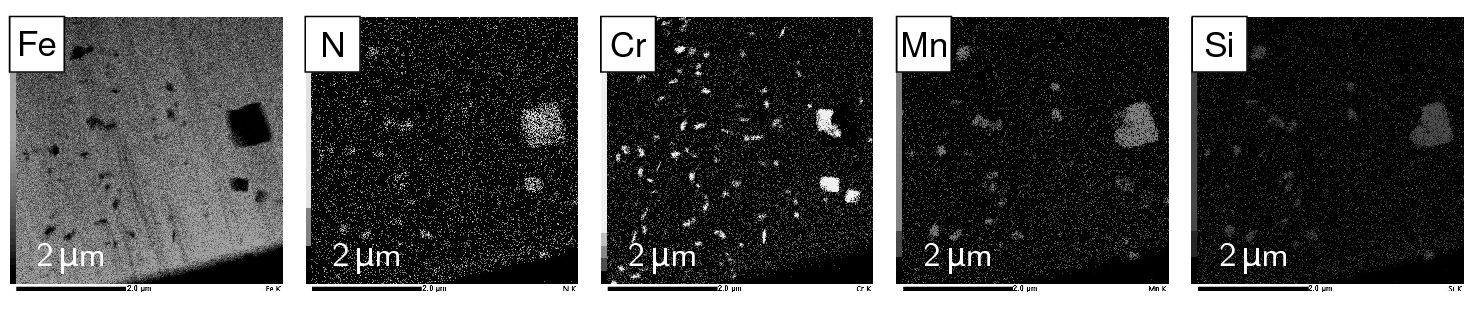
\includegraphics{figures/ch-04-TEM/x-tem_auto_cartography/figure.png}} % digital
  }
  
  \caption{\label{fig:chemical-maps-auto}Cartographie d'émission des rayons x caractéristiques des éléments constituant les nitrures de type \ch{MN} (avec \ch{M} majoritairement \ch{Cr}) et de type \ch{MnSiN2} formés pendant la carbonitruration de l'alliage 23MnCrMo5. Fraction massique en azote de 0,80\% en poids dans la région analysée.}
\end{figure}

\subsection{Alliage 16NiCrMo13 nitruré}

\begin{figure}[!b]
  \centering\resizebox{0.98\textwidth}{!}{
    \iftoggle{paper}
    {\includegraphics{figures/ch-04-TEM/x-tem_aero_cartography/figure.pdf}} % print
    {\includegraphics{figures/ch-04-TEM/x-tem_aero_cartography/figure.png}} % digital
  }
  
  \caption{\label{fig:chemical-maps-aero}Cartographie d'émission des rayons x caractéristiques des éléments constituant les nitrures de type \ch{MN} (avec \ch{M} majoritairement \ch{Cr}) formés pendant la nitruration de l'alliage 16NiCrMo13. Fraction massique en azote de 0,25\% en poids.}
\end{figure}

Comme pour la nuance 23MnCrMo5, la redistribution des éléments d'alliage lors de l'enrichissement en azote a été observée par analyse d'émission des raies de rayons x pour l'alliage 16NiCrMo13 nitruré. Dans le cas de cet alliage, seuls des nitrures de type \ch{MN} ont été observés (Figure~\ref{fig:chemical-maps-aero}), en accord avec la prédiction faite par Thermo-Calc~\cite{Andersson2002,Borgenstam2000} à l'aide de la base de données TCFE7, pour la composition de la lame observée.  Ces précipités, de morphologie globulaire ou sous forme de bâtonnet, couvrent une surface entre 1,8\% et 2,5\% de la section transversale des lames. Dès que les régions où les cartographies ont été réalisées atteignent une épaisseur moyenne de \SI{80}{\nano\metre} et si l'on suppose que tous les précipités \ch{MN} dans le volume sont détectés, alors une estimation de leur fraction volumique peut être faite par analyse d'images. On obtient qu'entre 0,8\% et 1,0\% de précipités sont formés. Thermo-Calc~\cite{Andersson2002,Borgenstam2000} prédit une fraction volumique autour de 1,0\% pour la composition locale, ce qui est assez proche de la valeur estimée par analyse des cartographies de rayons x. Cela implique une précipitation à l'équilibre dans la région étudiée et cela sert à valider l'approche du modèle de durcissement établi pour expliquer la dureté après trempe: les précipités attendus sont déjà formés et donc la prédiction de l'azote dissous dans la martensite est raisonnable.

%\pagebreak

La structure martensitique après trempe et traitement cryogénique de la nuance 16NiCrMo13 après nitruration en phase austénitique a été identifiée comme étant composée de lattes de largeurs typiques allant de \SIrange{200}{500}{\nano\metre} dans une région contenant 0,13\%~C et 0,25\%~N en poids. Ces structures sont présentées Figure~\ref{fig:tem-aero-micro-laths} où le contraste permet de visualiser quelques nitrures \ch{MN} identifiés Figure~\ref{fig:chemical-maps-aero}. L'alliage présente encore (Figure~\ref{fig:tem-aero-micro-shear}-b) des zones de cisaillement d'environ \SI{100 x 10}{\nano\metre} orientées dans deux directions possibles de la martensite, lesquelles sont probablement formées pendant la trempe. Ces zones correspondent à la structure ordonnée \ch{Fe16N2} et un détail de leur morphologie est présenté en haute résolution Figure~\ref{fig:tem-aero-micro-shear}-d, d'où le cliché de diffraction de la Figure~\ref{fig:tem-aero-micro-shear}-c a été obtenu. Bien que ces régions puissent se comporter comme barrières au glissement des dislocations, elles ne permettent pas d'expliquer le comportement en durcissement observé lors du revenu. Cela vient du fait que ces zones de cisaillement ont aussi été observées avant le revenu. %, juste après enrichissement.

\begin{figure}[h]
  \centering\resizebox{0.6\textwidth}{!}{
    \iftoggle{paper}
    {\includegraphics{figures/ch-04-TEM/x-tem_aero_mesoscale-laths/figure.pdf}} % print
    {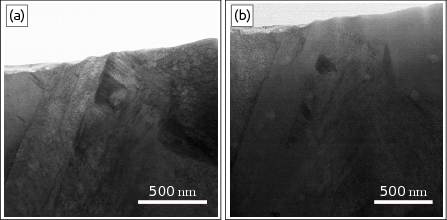
\includegraphics{figures/ch-04-TEM/x-tem_aero_mesoscale-laths/figure.png}} % digital
  }

  \caption{\label{fig:tem-aero-micro-laths}Micrographies de l'alliage 16NiCrMo13 nitruré, trempé et soumis au traitement cryogénique: (a) fond clair en mode STEM, mettant en évidence la structure martensitique en lattes ($\times$120k), (b) nitrure \ch{MN} formé à la température d'enrichissement (grandissement de $\times$100k).}
\end{figure}

Les structures de la Figure~\ref{fig:tem-aero-micro-shear} sont prises comme état de référence pour l'étude des échantillons soumis au revenu au-dessus de \SI{573}{\kelvin}: on cherche des caractéristiques pour ces dernières qui ne sont pas présentes avant le revenu. On vérifie Figure~\ref{fig:tem-aero-nano} dans la matrice martensitique cubique centrée de l'alliage 16NiCrMo13 nitruré et soumis au revenu à \SI{573}{\kelvin} la présence d'une multitude de précipités nanométriques \textendash{} moins de \SI{5}{\nano\metre} \textendash{} qui n'ont pas été détectés dans la lame correspondant à la Figure~\ref{fig:tem-aero-micro-shear}. En raison de leur taille et de leur cohérence avec la matrice, ces nitrures sont possiblement à l'origine du comportement en durcissement mis en évidence Figure~\ref{fig:hardness_nitriding} après nitruration austénitique et revenu au-dessus de \SI{573}{\kelvin}. Il est donc probable que la martensite alliée à l'azote présente un comportement similaire à celui du fer pur où la décomposition \ch{Fe16N2 -> Fe4N}~\footnote{Il doit être clair que cette décomposition n'est pas st{\oe}chiométrique: \ch{Fe16N2} est une structure ordonnée métastable avec environ deux fois le paramètre de maille de la ferrite qui se décompose pour donner du nitrure \ch{Fe4N} et de la ferrite $\alpha$ à l'équilibre.} serait retardée en température \textemdash{} du fait que des précipités de type \ch{Fe4N} n'ont pas été détectés. Cette transition pourrait aussi être limitée par la cinétique, du fait de la faible teneur en azote ajouté à l'alliage comparée à celle rapportée par \citet{Kaplow1983} qui ont mis en évidence la formation de \ch{Fe4N} à \SI{433}{\kelvin}.

\begin{figure}[h]
  \centering\resizebox{0.6\textwidth}{!}{
    \iftoggle{paper}
    {\includegraphics{figures/ch-04-TEM/tem_aero_mesoscale-shear/figure.pdf}} % print
    {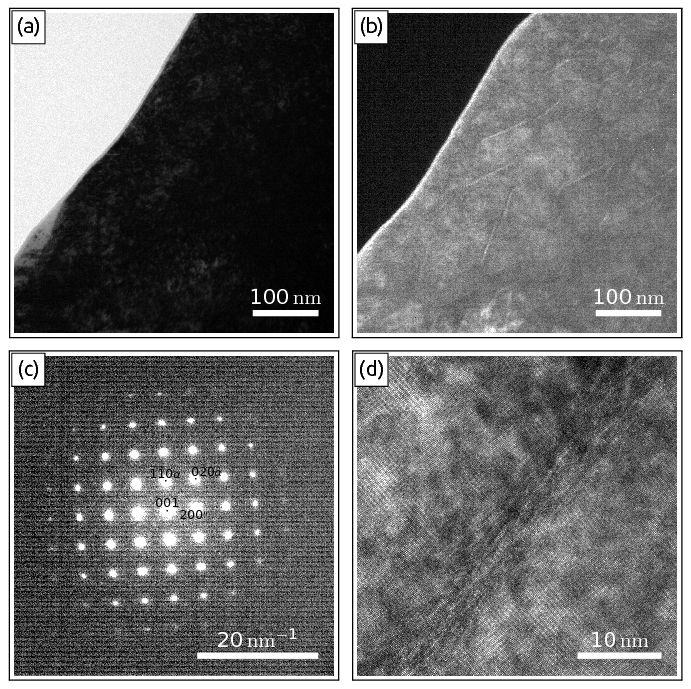
\includegraphics{figures/ch-04-TEM/tem_aero_mesoscale-shear/figure.png}} % digital
  }
  
  \caption{\label{fig:tem-aero-micro-shear}Micrographies de l'alliage 16NiCrMo13 nitruré, trempé à l'huile et à l'azote liquide: (a) fond clair (BF) orienté en position de diffraction, (b) même région en fond sombre (DF) selon l'axe de réflexion [001] (c) cliché de diffraction et (d) image en haute résolution (HRTEM) des zones \ch{Fe16N2} (grandissement de $\times$2M).}
\end{figure}

\begin{figure}[h]
  \centering\resizebox{0.6\textwidth}{!}{
    \iftoggle{paper}
    {\includegraphics{figures/ch-04-TEM/tem_aero_nanoscale/figure.pdf}} % print
    {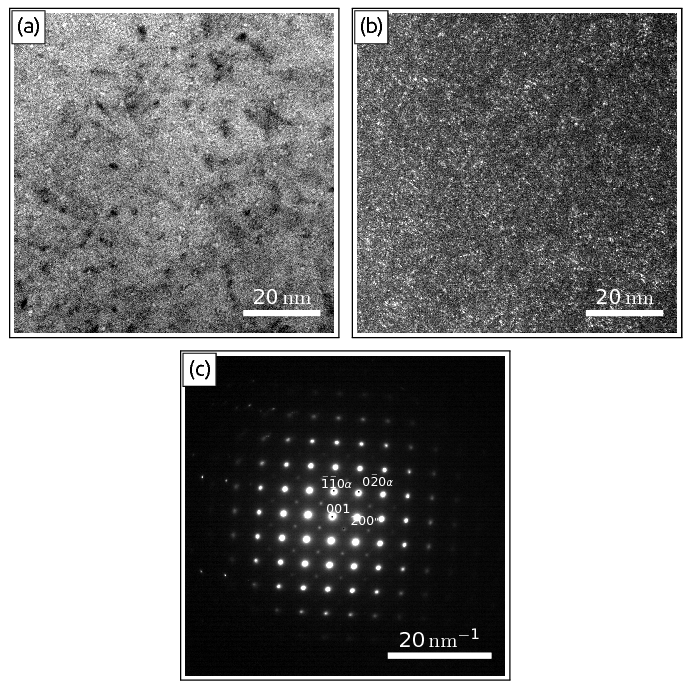
\includegraphics{figures/ch-04-TEM/tem_aero_nanoscale/figure.png}} % digital
  }
  \caption{\label{fig:tem-aero-nano}Échantillon de la Figure~\ref{fig:tem-aero-micro-shear} après revenu à \SI{573}{\kelvin}: (a) image en fond clair (BF) d'une région contenant une forte densité de nano-précipités (b) même région en fond sombre (DF) où les précipités orientés apparaissent comme des points clairs et (c) SAED de la région avec cliché de diffraction des précipités \ch{Fe16N2}.}
\end{figure}

\clearpage\section{Conclusion}

Le Chapitre~\ref{ch:reponse_metallurgique} fait état des expériences qui ont été réalisées à pression atmosphérique pour caractériser la réponse métallurgique des alliages 16NiCrMo13 et 23MnCrMo5, principalement en ce qui concerne le rôle de l'azote dans les traitements thermochimiques réalisés en phase austénitique. Les principales observations présentées dans ce chapitre sont les suivantes:
\begin{itemize}
  \item les prises de masse évaluées du moyen d'une balance de précision~\footnote{De l'ordre de \SI{0,1}{\milli\gram}.} ou par intégration des profils de diffusion mesurés par micro-sonde se trouvent en accord avec les simulations pour une saturation en carbone à la surface des pièces traitées. En ce qui concerne l'azote, l'alliage 23MnCrMo5 reproduit bien la condition à la limite prédite d'activité $a_{\ch{N}}^{m}=40$. Cependant, la nuance 16NiCrMo13 présente des difficultés d'enrichissement en azote avec une composition en surface associée avec une activité $a_{\ch{N}}^{m}=10$ dans l'atmosphère et conduit à une décarburation moins intense. Ceci a été attribué à un possible effet de catalyse sur la recombinaison des atomes issus de la décomposition de l'ammoniac;
  
  \item la trempe à l'huile de la nuance 16NiCrMo13 produit des fractions importantes en austénite résiduelle pour des teneurs en interstitiels au--delà du point--H; le traitement cryogénique par immersion dans l'azote en ébullition a permis de transformer presque complètement cette phase $\gamma_{R}$ en martensite $\alpha^{\prime}$; les filiations de dureté des matériaux après trempe à l'huile et traitement cryogénique ont été reliées à la composition locale en négligeant le gradient de microstructure \textendash{} seule la contribution des interstitiels a été prise en compte dans le modèle de durcissement, Équation~\ref{eq:norstrom_model} \textendash{} et montrent une bonne adéquation avec ce modèle. L'incorporation de l'azote pour expliquer les duretés obtenues après trempe a été possible grâce aux simulations de l'équilibre réalisées à l'aide de Thermo-Calc~\cite{Andersson2002,Borgenstam2000} qui ont permis d'estimer la fraction en azote dissous dans la martensite après trempe;
  
  \item la tenue en dureté après revenu des pièces carbonitrurées s'avère être meilleure que celle des pièces cémentées, cela étant évident pour l'alliage 23MnCrMo5 qui gagne \SI{70}{\HV} supplémentaire dans la région riche en azote; dans le cas de la nitruration, la preuve d'une précipitation secondaire de \ch{Fe16N2} dans la profondeur enrichie est observée;
  
  \item des investigations par TEM ont mis en évidence des nitrures de type \ch{MN} pour les deux nuances; la nuance 23MnCrMo5 présente aussi des nitrures \ch{MnSiN2}, qui ne sont pas inclus dans la base de données utilisée pour simuler l'alliage; les effets observés lors du revenu des alliages enrichis en azote ont été attribués à une fine précipitation de \ch{Fe16N2} qui a lieu à l'échelle nanométrique.
\end{itemize}

\endinput